\documentclass[a4paper, 12pt]{article}
\usepackage[slovak]{babel}
\usepackage[utf8]{inputenc}
\usepackage{lmodern}
\usepackage[T1]{fontenc}
\usepackage{slovak}				%obsahuje slovenske znaky, ktore sa nenachadzaju v standardnom baliku
\usepackage{algorithm}%[section]{algorithm}
\usepackage{algorithmic}
%\usepackage{cite}
\usepackage{graphicx}			% pre vkladanie obrazkov \includegraphics
\usepackage{subfig}				
\usepackage{courier}			% \textt{} bude zodpovedat pismu Courier
\usepackage{float}				% plávajúce objekty/obrázky, možné použiť parameter "H" pre príkaz figure
\usepackage{chngcntr}			% Na číslovanie objektov. (Defines commands \counterwithin (which sets up a counter to be reset when another is incremented) and \counterwithout (which unsets such a relationship)).
\usepackage{pdflscape}			% lanscape mod
\usepackage{amsmath}
\usepackage{amsfonts}
\usepackage{geometry}			% pre rozmery stran a pod.

%\usepackage{url}
\usepackage{hyperref}			% klikatelne krizove odkazy na kapitoly, obrazky, referencie
	\hypersetup{colorlinks,				%linky budu farebne
    	citecolor=black,						%citacie cierne
    	filecolor=black,
    	linkcolor=black,						%
    	urlcolor=blue,							%url budu modre
    	}    	

\counterwithin{equation}{section} % Cislovanie rovnic bude obsahovat c. kapitoly a poriadie rovnice v danej kapitole, pre tento prikaz musi byt package "chngcntr"
 	
\linespread{1.3}					% riadkovanie 1,5
%\linespread{1.4}

\floatname{algorithm}{Algoritmus} 	% zmeni prostredie \algorithm na slov. Algoritmus
%\newtheorem{Algoritmus}{Algoritmus}[section]

\begin{document}

%\title{My Article}
%\author{Nobody Jr.}
%\date{Today}
%\maketitle
%\newpage

%%\topmargin = 1cm
\begin{titlepage}
	\begin{center}
	\large Slovenská technická univerzita v Bratislave 
	\normalsize \\
\large Fakulta informatiky a informačných technológií
	\end{center}
	\begin{center}
	  FIIT-5212-56275
	\end{center}
	\vfill
	\begin{center}
	
\begin{center}
\Large Bc. Pavol Pidanič
\end{center}
	
\begin{center}
\LARGE \textbf{Vyššie schopnosti hráča simulovaného robotického futbalu}
\end{center}
\begin{center}
\large Diplomová práca
\end{center}
\linespread{1.3}
	\end{center}
	\vfill
	Vedúci práce: Ing. Ivan Kapustík \\\\
	máj 2014
\end{titlepage}

%%\documentclass{article}
%\usepackage[cp1250]{inputenc}
%\usepackage[slovak]{babel}

%\begin{document}
\begin{titlepage}
	\begin{center}
	\large Slovenská technická univerzita v Bratislave \\ \Large Fakulta informatiky a informačných technológií
	\\ \large FIIT-5212-56275
	\end{center}
	\vfill
	\begin{center}
	\Large Bc. Pavol Pidanič \\
	\LARGE \textbf{Vyššie schopnosti hráča simulovaného robotického futbalu} \\
	\large Diplomová práca
	\end{center}
	\vfill
	\small
	\textbf{Študijný program:} Softvérové inžinierstvo \\
	\textbf{Študijný odbor:} 9.2.5 Softvérové inžinierstvo \\
	\textbf{Miesto vypracovania:} Ústav informatiky a softvérového inžinierstva, Fakulta informatiky a informačných technológií, Slovenská technická univerzita v Bratislave \\
	\textbf{Vedúci práce:} Ing. Ivan Kapustík \\\\
	máj 2014
	\normalsize
\end{titlepage}
%\end{document}
%\begin{titlepage}
\large\textbf{Anotácia}\\\\
\normalsize
Slovenská technická univerzita v Bratislave \\
FAKULTA INFORMATIKY A INFORMAČNÝCH TECHNOLÓGIÍ \\
Študijný program: Softvérové inžinierstvo \\
\\
Autor: Bc. Pavol Pidanič \\
Diplomový projekt: Vyššie schopnosti hráča simulovaného robotického futbalu \\
Vedenie diplomového projektu: Ing. Ivan Kapustík \\ 
máj 2014 \\
\\
Práca je venovaná svetovej iniciatíve RoboCup, ktorej cieľom je podpora rozvoja robotiky a umelej inteligencie. Simulovaná robotická 3D liga je časť tejto problematiky, ktorej sa venujú aj výskumníci na Fakulte a informatiky a informačných technológií. Na začiatku opisujeme fakultného hráča s menom JIM a stav riešenia za posledné roky diplomovými prácami a na predmete Tímový projekt. Práca sa zameriava na problém riešenia dynamického kopu. Obsahuje opis riešení najlepších svetových tímov a tímov, ktoré sa venujú hlavne dynamickému a parametrizovateľnému kopu. V popise návrhu uvádzame algoritmus implementácie takého kopu jedného zo svetových tímov a poznatky získané z aktuálneho stavu fakultného hráča súvisiace s návrhom dynamického kopu.

%Práca je venovaná metódam celočíselnej optimalizácie v úlohách prediktívneho riadenia hybridných systémov. Riešenie úloh celočíselnej optimalizácie je zložitý kombinatorický problém, v ktorom počet možných riešení exponenciálne narastá s počtom parametrov optimalizačnej úlohy. V práci je opísaná metóda vetiev a hraníc, ktorej výhodou je redukcia prehľadávaného priestoru prípustných riešení. Implementovaný algoritmus tejto metódy je využitý v prediktívnom riadení hybridných systémov. Algoritmus prediktívneho riadenia využíva hybridný model systému pre predikciu vývoja systému. Na základe získanej predikcie je riešená celočíselná optimalizačná úloha, ktorej výstupom je optimálny riadiaci zásah. Funkcia algoritmu je demonštrovaná na probléme riadenia dynamického systému satelitu. 

\end{titlepage}
%\begin{titlepage}
\large \textbf{Annotation} \\ \\
\normalsize
Slovak University of Technology Bratislava \\
FACULTY OF INFORMATICS AND INFORMATION TECHNOLOGIES \\
Degree Course: SOFTWARE ENGINEERING  \\
 \\
Author: Bc. Pavol Pidanič \\
Diploma Project: Kick skills augmentation for a simulated robotic soccer player \\ 
Supervisor: Ing. Ivan Kapustík  \\
2015, May \\
\\
The main topic of this thesis is world initiative RoboCup. RoboCup's goal is to support a development of a robotics and artificial intelligence. Simulated 3D robotic soccer league is part of RoboCup initiative and it is in the aim of researchers at Faculty of informatics and information technologies. In the beginning we start with the description of the faculty robot, named JIM and the actual achieved progress. The goal of this thesis is kick skills augmentation for a simulated robotic soccer player. We examined directional kicks and their dependencies to different parameters. Based on our experiments we created 4 new directional kicks. A forward and inverse kinematics module is also part of this thesis.


%Práca je venovaná svetovej iniciatíve RoboCup, ktorej cieľom je podpora rozvoja robotiky a umelej inteligencie. Simulovaná robotická 3D liga je časť tejto problematiky, ktorej sa venujú aj výskumníci na Fakulte a informatiky a informačných technológií. Na začiatku opisujeme fakultného hráča s menom JIM a stav riešenia za posledné roky diplomovými prácami a na predmete Tímový projekt. Práca sa zameriava na problém riešenia rozšírenia schopnosti kopania hráča. Skúmali sme spôsoby vykonania kopu do strany na základe rôznych parametrov. Na základe experimentov sme vytvorili 4 rôzne kopy do strany. Súčasťou práce je aj modul pre doprednú a inverznú kinematiku.

\end{titlepage}

\pagenumbering{Roman}			% číslovanie strán rímskymi číslami (kapitálky)
%\tableofcontents				% obsah
%\newpage

%\listoffigures					% zoznam obrázkov
%\newpage
%\listoftables					% zoznam tabuliek
%\newpage

\pagenumbering{arabic}			% číslovanie strán arabskými číslami
%\section{Úvod}

Agentovo-orientované programovanie \cite{shoham} je založené na kognitívnom a sociálnom pohľade na softvér. Agentom sa nazýva softvérová entita, ktorá sa správa autonómne a nezávisle v dynamicky a nepredvídateľne sa meniacom prostredí, v ktorom koexistujú aj iné agenty.

Jedným z príkladov agentovo-orientovaného návrhu softvéru je simulovaná futbalová liga robotov - RoboCup.
RoboCup \cite{robocup} je svetová iniciatíva, ktorá vznikla v roku 1997. Snaží sa podporiť povedomie verejnosti o robotike a umelej inteligencii. Cieľom je podporiť vedecký výskum. Podporou výskumu a organizovaním súťaži sa zameriava na dosiahnutie hlavného cieľa. Tým je vytvoriť do roku 2050 tím autonómnych hráčov, ktorí dokážu poraziť aktuálnych majstrov sveta vo futbale podľa medzinárodnej futbalovej federácie FIFA. Menším cieľom je vytvoriť tím robotov, ktorí dokážu hrať ako ľudskí hráči. 

V rámci tohto projektu existujú viaceré ligy deliace sa podľa typu používaných hráčov a spôsobu  realizácie  zápasov.  Jedná  sa  napríklad  o ligu  humanoidných  robotov,  ligu  stredne veľkých  robotov,  ligu  malých  robotov,  ligu  štandardnej  platformy  a  simulovanú  ligu. Spomínané  ligy  sa  ešte členia  podľa  rôznych  kritérií. Fakulta informatiky a informačných technológií sa zameriava na simulovanú trojrozmernú ligu. 

Predlohou hráča simulovanej ligy je humanoidný robot Nao vyrábaný spoločnosťou Aldebaran Robotics\footnote{\url{http://www.aldebaran.com/}}. Jeho výška je $57~cm$ a hmotnosť $4,5~kg$. Má 22 kĺbov – 6 na nohe, 4 na ruke a 2 na krku. Zápas prebieha v prostredí so simulovaným fyzikálnym modelom. Ako simulačné prostredie sa využíva server Simspark\cite{simspark}. Hráči komunikujú so serverom v $20~ms$ intervaloch pomocou TCP/IP protokolu. Hráč prijíma informácie o prostredí pomocou senzorov – perceptorov. Poskytujú informácie o postavení a orientácii hráča v prostredí, natočení kĺbov, silách, ktoré pôsobia na robota. Hráč z prostredia prijíma aj vizuálne a zvukové vnemy. 

Hráč  odosiela  serveru  príkazy  na  zmenu polohy  jednotlivých  kĺbov.  Simultánnou  zmenou  natočenia  viacerých  kĺbov  sa  dosahuje jednoduchý pohyb hráča. Tzv. nižšie schopnosti, ako je chôdza, otáčanie alebo kopnutie do lopty, vznikajú kombináciou týchto pohybov. Vyššie pohyby sa skladajú z nižších a vyberajú sa na základe stavu agenta. Na najvyššej úrovni je taktika. Od vyspelosti taktiky tímu závisí celková hra, aj schopnosť vyhrať nad súperom. 

\subsection{Štruktúra práce}
Práca sa člení na tieto časti. Práca nadväzuje na ostatné práce na fakulte a preto v kapitole \ref{sec_analysis} sú popísané doterajšie výsledky - tímové projekty a diplomové práce. Kapitola \ref{sec_current} opisuje aktuálny stav hráča a ciele, ktoré by sme chceli dosiahnuť. Kapitola \ref{sec_specification} vyjadruje, ktoré získané poznatky sme sa rozhodli využiť a taktiež popisuje návrh prototypu. V kapitole \ref{sec_implementation} opisujeme implementáciu vytvoreného prototypu. Na to nadväzuje kapitola \ref{sec_verification} s popisom testovacích prípadov prototypu. Doterajšie výsledky a ďalšiu prácu zhodnotíme v kapitole \ref{sec_conclusion}.
%\newpage

%\section{Analýza problémovej oblasti}
V tejto časti analyzujeme práce dokončené na Fakulte informatiky a informačných technológií a prístupy najlepších svetových tímov, ktoré sa venovali najmä parametrizovateľnému a dynamickému kopu.

\subsection{Práce na FIIT}

Táto práca nadväzuje na výsledky vytvorené v minulých rokoch na Fakulte informatiky a informačných technológií (FIIT). Simulovanej robotickej lige sa venovali a venujú bakalárske, diplomové a tímové projekty. Opíšeme si architektúru fakultného hráča a zhrnieme si práce dokončené v poslednom období a hlavne uvedieme to najdôležitejšie, čo sa vykonalo pri vytváraní kopových vlastností fakultného robota.

%\subsubsection{Hráč JIM}
	\label{jim}
Aktuálnou predlohou hráča, vyvíjanou aj na predmete Tímový projekt, z ktorej bude vychádzať táto práca, je verzia agenta s názvom JIM. Jeho autormi sú 3 absolventi FIIT v roku 2011 - Juraj Drahoš, Ivan Hujsi, Maroš Urbanec. Zo začiatočných písmen ich mien je vytvorený aj názov JIM.

Jadro robota je napísané v objektovo-orientovanom jazyku Java. Jadro tvorí aj najväčšiu časť robota. %Pre rozhodovanie a používané schopnosti sú použité Ruby skripty. Pretože jazyk Ruby je interpretovaný jazyk, hráč dokáže načítať súbory pohybov za behu. Ďalšou výhodou Ruby je možnosť meniť parametre pohybu alebo správania bez nutnosti prekompilovať zdrojový kód.

Architektúra agenta je založená na modeli Believe Desire Itention (BDI). Ide o decentralizovanú architektúru, často využívanú v multiagentových prostrediach. Agent  si  na  základe  získaných  vnemov  utvorí  predstavu  o  okolitom   svete  a  na  základe existujúcej  situácie  a  cieľov  si  vytvorí  plán.  Pri  rozhodovaní  sa  teda  riadi  aktuálnym stavom  sveta  a stanovenými  cieľmi.  Úlohou  plánovača je  vytvoriť  plán  zodpovedajúci  obom kritériám.

Architektúra robota JIM pozostáva z 5 komponentov:

\begin{itemize}
	\item \textit{Model komunikácie} - úlohou je komunikovať so serverom a zabezpečovať analýzu správ
	\item \textit{Model parsovania} - parsuje prijaté správy zo servera
	\item \textit{Model sveta} - predstavuje v architektúre BDI časť Believe. V súčasnom stave je rozdelený na 3 časti. Jednotlivé časti sa aktualizujú samostatne na základe správ prijatých zo servera.
		\begin{itemize}
			\item \textit{Agent model} - obsahuje informácie o pozícii hráča, jeho rotácií, rýchlosti a natočení kĺbov.
			\item \textit{World model} - v ňom sa spracúvajú informácie o lopte - jej rýchlosti a pozícii na ihrisku. Ďalšími informáciami sú pozície, rýchlosti ostatných hráčov.
			\item \textit{Environment model} - informácie o hre.
		\end{itemize}
	\item \textit{Plánovací modul} - v architektúre BDI predstavuje časť Desire a Intention. Skladá sa z dvoch častí. Tými sú plánovací algoritmus a vyššie schopnosti. Plánovací algoritmus je možné jednoducho meniť, vďaka spôsobu, akým je architektúra navrhnutá.
	\item \textit{Modul pohybov} - vykonáva požadované pohyb, ktoré dostáva ako príkazy z vyšších schopností a na základe modelu sveta.
\end{itemize}

Tieto komponenty sú navzájom prepojené. Schému architektúry hráča a prepojenie modulov zobrazuje obrázok \ref{pic_jim_architecture}.

\begin{figure}[H]
	\center
	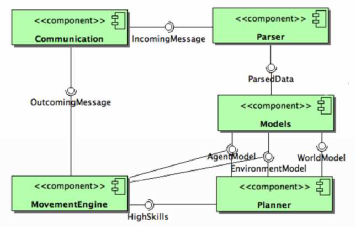
\includegraphics[scale=1]{./data/jim_architecture}
	\caption{Architektúra hráča JIM \cite{durcak}}
	\label{pic_jim_architecture}
\end{figure}

%\subsection{Diplomové práce v roku 2013}
\subsubsection{Diplomová práca Lukáša Ďurčáka} \label{sec_durcak}

Diplomová práca Lukáša Ďurčáka\cite{durcak} je jednou z dvoch dokončených prác v roku 2013.

Autor sa v nej venoval rozšíreniu vyšších schopností hráča - rozhodovanie a zhodnotenie situácie na ihrisku. Pri vyšších schopnostiach sa zameral na schopnosť agenta odhaliť kolízie medzi hráčom a prekážkou, alebo hráčom a ďalším hráčom a vytvoril systém, ako týmto situáciám predísť. Hráč je schopný obchádzať protihráčov a ostatné prekážky a tak nebude dochádzať k neželaným pádom. Pri riešení kolízií sa rozhodol využiť analytickú geometriu. Aj keď zápasy simulovanej ligy prebiehajú v trojrozmernom priestore, každá ním riešená situácia sa dá pretransformovať do jednoduchších útvarov v dvojrozmernom priestore. Do modelu kolízií je zarátaná aj predikcia pohybu hráčov. Táto schopnosť dokáže určiť približný smer a rýchlosť pohybu ostatných hráčov na ihrisku. 

Vlastnosťou, ktorá súvisí so zameraním práce, je rozhodovanie výberu miesta na kopnutie, teda prihrávku. Hráč sa rozhoduje, či kopne loptu smerom na bránu, pokúsi sa prihrať alebo bude driblovať na vhodnejšie miesto. Hráč vykoná kop na bránu, ak sa medzi ním a bránou nenachádza žiadna prekážka a je v dostatočnej vzdialenosti od brány. Dostatočná vzdialenosť je taká, ak je menšia ako vzdialenosť, ktorú je možno dosiahnuť kopom. Pri kopaní na bránu sa nesústredí na stred brány, ale berie do úvahy aj postavenie súperovho brankára. Prihráva v takom prípade, ak je vzdialenosť od brány väčšia ako dokáže kopnúť a ak existuje prekážka, ktorá bráni kopnutiu.

Hráča rozšíril o schopnosti tímovej hry. Jednou zo schopností je komunikácia medzi hráčmi. Hráči si dokážu medzi sebou posielať správy a získavať z nich informácie. Ďalšou doplnenou schopnosťou je spôsob hrania vo formáciách. Vytvoril a otestoval niekoľko rôznych formácií. Formácie rozlišujú defenzívnu alebo ofenzívnu pozíciu hráča.

Nakoniec vytvoril testovací nástroj. Umožňuje vytváranie herných situácií. Agent sa môže na ihrisku správať na základe umelo vytvorenej hernej schémy. Slúži na lepšie pochopenie činností a rozhodnutí, ktoré hráč vykonáva pomocou dostupných informácií z prostredia.

%\subsubsection{Diplomová práca Petra Paššáka} \label{sec_passakp}
Ide o druhú dokončenú prácu v roku 2013. V nej sa zameral na vylepšenie už existujúcich pohybov robota pomocou evolučných algoritmov. Pohyby, ktorým sa venoval boli kopy do lopty, chôdza vpred a vzad a úkroky do strany \cite{passak_peter}.

Predtým ako sa pustil do vylepšovania, upravil jemu dostupné testovacie prostredie, aby poskytovalo používateľské rozhranie, ktoré zaznamenávalo metriky, mohlo nastavovať parametre testovania a aby bolo možné vyhodnocovať výsledky.

Pre skúmané pohyby si určil ich kvalitu, ktorú sa snažil dosiahnuť.
\begin{itemize}
	\item stabilita pre všetky pohyby
	\item vzdialenosť, ktorú prejde za určitý čas a vychýlenie z trasy pre chôdzu
	\item vzdialenosť a vychýlenie zo smeru pre kopy
\end{itemize}

Pri kopoch si zvolil pohyb \texttt{shot\_left}. Z pôvodnej priemernej vzdialenosti $4,4~m$ a maximálnej vzdialenosti $4,7~m$ dosiahol hodnoty v priemere $9,21~m$ a dosiahnuté maximum bolo $10,65~m$. Tieto dĺžky kopov zodpovedajú vzdialenosti od stredového kruhu až k bráne.

Pri chôdzi bol zvolený pohyb \texttt{walk\_fine2\_optimized2}. Tento pohyb však mal pri vylepšovaní problémy so stabilitou pri rozbehu chôdze. Preto vytvoril nový pohyb pod menom \texttt{turbo\_walk}, ktorý rozšíril o fázu úkrokov pravej a ľavej nohy. Pôvodnú rýchlosť chôdze $0,32~ms^{-1}$ vylepšil na výsledných $0,97~ms^{-1}$ pri  $80\%$ stabilite. So $100\%$ stabilitou chôdza dosahovala rýchlosť $0,68~ms^{-1}$.

Chôdzu vzad \texttt{walk\_back} vylepšil z $0,1~ms^{-1}$ na $0,54~ms^{-1}$ pri $92\%$ stabilite. A pri úkrokoch do strany \texttt{stepleft\_new\_smaller} z pôvodnej rýchlosti $0,05~ms^{-1}$ dosiahol rýchlosť $0,09~ms^{-1}$ so $100\%$ stabilitou a $0,16~ms^{-1}$ s úspešnosťou $93\%$.

%\subsubsection{Staršie diplomové práce}\label{sec_auder_hudec}

V tejto časti popíšeme výsledky starších prác na FIIT ako už spomenuté diplomové práce Lukáša Ďurčáka (kapitola \ref{sec_durcak}) a Petra Paššáka (kapitola \ref{sec_passakp}) pridané do implementácie robota JIM (kapitola \ref{jim}). V niektorých prácach dosiahli zrýchlenie niektorých pohybov. Avšak tieto výsledky nebudeme uvádzať, pretože pohyby boli optimalizované v práci Petra Paššáka (kapitola \ref{sec_passakp}).

Miloš Auder vo svojej práci\cite{auder} z roku 2012 skúmal prístupy ku chôdzi, spôsoby hľadania cesty a tiež metódy ako genetické algoritmy, strojové učenie a ich následné využitie v doméne Robocup. Vytvoril nové otáčanie hráča na mieste, ktoré je možné parametrizovať, a tak dosiahnuť väčší uhol natočenia. Vznikol aj nový typ chôdze s tzv. ľudským výzorom. Avšak efektívna bola len na kratšie vzdialenosti. Pri hľadaní cesty vznikli 2 prístupy. Jedným je priblíženie hráča k lopte. Pri druhom prístupe, v ktorom sa hráč snaží prejsť oblasť so súperovými hráčmi, použil genetický algoritmus. Výsledkom sú body, cez ktoré má hráč prejsť.

Ďalším autorom v roku 2012 je Ján Hudec\cite{hudec}. Zameral sa na stabilizačné funkcie a ovládače pre chôdzu. Pri stabilizácii využil hodnoty Zero Moment Point a informácie o pozícii tela robota zapracovaním vyhodnocovania Force Resistance (FR) perceptora.

Poslednou diplomovou prácou v roku 2012 je práca Martina Paššáka. Tá úzko súvisí s prácou jedného z autorov hráča JIM - Ivana Hujsiho. Obaja sa venovali pohybom robota. 

Ivan Hujsi\cite{Hujsi} navrhol a vytvoril 19 nových pohybov. Z toho bolo 11 kopov určených na prihrávanie a streľbu pri rôznych pozíciách lopty. Vznikli pohyby na posúvanie a napravovanie lopty a tiež niekoľko základných pohybov ako chôdza, vstávanie z brucha a chrbta. Tieto pohyby boli vytvorené ručne bez použitia automatických nástrojov. Tiež navrhol a implementoval algoritmus výberu smeru kopnutia.

Už z názvu práce Martina Paššáka\cite{passak_martin} vyplýva, že sa zameral na spôsoby, ako hráč manipuluje s loptou. Vo výsledkoch vylepšil zatáčajúcu chôdzu, pri ktorej robot dynamicky upravuje smer chôdze zmenou kroku. Bol pridaný modul, s ktorým je možné zrýchľovať a spomaľovať chôdzu. Upravil približovanie k lopte a taktiež upravil obchádzanie lopty. Vytvoril chôdzu s loptou na určené miesto. Pri kopaní vytvoril nové pohyby a model, ktorým je možné kopy parametrizovať. Na záver prepracoval hlavný plán hráča, ktorý využíva rozhodovací strom. Tým dosiahol jednoduchšie rozhodovanie hráča.

%\subsection{Tímové projekty}

\subsubsection{A55Kickers}\label{A55Kickers}

Tím A55Kickers \cite{A55Kickers} je jediným tímom v roku 2012, ktorý sa venoval problematike simulovaného futbalu počas predmetu Tímový projekt. 
% Zároveň je aj najaktuálnejším tímom, ktorý odovzdal kompletnú dokumentáciu.\footnote{V akademickom roku 2013/2014 v predmete Tímový projekt sa problematike RoboCup venujú 2 tímy. Počas písania práce prebieha výučba v letnom semestri a predmet nie je uzavretý. Preto sme sa rozhodli, že výsledky tímov Megatroll a Gitmen doplníme, keď tímy odovzdajú celú dokumentáciu s výsledkami, ktoré dosiahli. Aktuálne informácie sú dostupné na oficiálnych stránkach tímov: Megatroll \url{http://team04-13.ucebne.fiit.stuba.sk/} a Gitmen \url{http://team09-13.ucebne.fiit.stuba.sk/}}

Jedným z ich výsledkov je práca na wiki stránke projektu\footnote{Aktuálne dostupná \url{http://labss2.fiit.stuba.sk/TeamProject/2013/team09is-si/wiki/index.html}}, ktorú zdedili od predchádzajúcich tímov High5 a Tím 17 žije. Po doplnení informácií o práci tímu vytvorili novú štruktúru wiki, ktorá podľa ich slov zabezpečuje ľahšiu orientáciu a rýchly prístup k informáciám. Štruktúra sa delí na 3 sekcie. Prvé dve obsahujú informácie o RoboCup iniciatíve a stave projektu na fakulte. Tretia sekcia je určená ako podpora ohľadom inštalačných záležitostí a používateľských príručiek projektu RoboCup na FIIT, ktoré sú nevyhnutné pre riešenie projektu.

Zamerali sa tiež na vylepšenie nižších pohybov (tzv. Low Skills). Vylepšili takmer všetky dovtedy existujúce pohyby od chôdze, presunov po ihrisku a taktiež kopnutia, ktoré stabilizovali a zrýchlili. Ďalej vytvorili nové pohyby - stabilné kopnutia rôznou silou, nové otáčania, úkroky rôznych veľkostí, dokonca aj efektívnejšie vstávania zo zeme. Kvôli prepojeniu vyšších zručností (High Skills), navrhli a implementovali základnú polohu agenta. Základná poloha je taká, do ktorej sa robot nastaví vždy po vykonaní pohybu. Je stabilnejšia a prirodzenejšia, pretože bod ťažiska bol posunutý nižšie. Všetky pohyby premenovali, aby ich pomenovania zodpovedali typu pohybu a ostatným parametrom pohybu. Upravené pohyby využili pri úpravách vyšších pohybov.

Upravili už existujúci pohyb \texttt{Kick}, ktorý by zodpovedal prihrávaniu. Pohybu doplnili parameter, ktorý slúži na zadanie miesta, na ktoré je potrebné kopnúť. Na výber sily kopu využili už existujúcu metódu pre určenie vzdialenosti lopty od požadovaného bodu.



%V závere naznačujú, kam by sa projekt na fakulte mohol ďalej uberať, %pretože robot nedosahuje vlastnosti hráčov svetovej úrovne. 
%------------------------------------------
%Z tohto dôvodu je do budúcnosti potrebné pracovať na zdokonaľovaní taktiky, vylepšovaní videnia sveta a v neposlednom rade aj na samotných pohyboch a stabilizácii agenta. Keďže súčasný fakultný agent ma implementované len statické pohyby je možne ho rozšíriť o dynamické pohyby, ktoré by mali zvýšiť rýchlosť agenta a tým zvýšiť jeho konkurencie schopnosť.
%Ďalším krokom by mohla byť stabilizácia agenta s využitím stabilizačných kritérií, ktoré by zabezpečili zníženie pádov pri hraní futbalu. Tiež sa dá pracovať na zdokonaľovaní taktiky, ktorá zatiaľ nie je v takom stave, aby odzrkadľovala hranie reálneho futbalu. V taktike sa dá pracovať na tvorbe prihrávok, nabiehaní na prihrávky, obchádzaní súpera a rôznych iných možnostiach
%----------------------------------------

%\subsubsection{High5 a Tím 17 žije}

Tieto tímy pracovali na fakultnom agentovi v predošlom akademickom roku ako tím A55Kickers, ktorý je opísaný v kapitole \ref{A55Kickers}.

Tím 17 žije\cite{tim17zije} vytvoril silný priamy kop, ktorý pozostáva z naváženia na jednu nohu, prikročenia druhou nohou, kopu prvou nohou a stabilizovaniu hráča. Pri chôdzi doplnili mierne prikrčenie a zrýchlenie na začiatku pohybu a pri ukončení chôdze jej spomalenie. Ďalej zabezpečili výber pohybov tak, aby sa agent dokázal natáčať a posúvať zároveň. Implementovali metódy pre nájdenie spoluhráčov a určenie, ktorý hráč je najbližšie k lopte. Hráč dokáže predpovedať pozíciu lopty a určiť vhodnosť prihrávky. Doplnili vyhodnotenie herných situácií, či je mužstvo pod tlakom alebo nie. Do testovacieho frameworku pridali grafické zobrazenie hry. V okne je možné zobraziť dáta o jednom alebo všetkých agentoch, o ich polohe a rotácií a informácie o polohe lopty.

Tím High5\cite{high5} vytvoril viacero úrovní kopu špičkou. Vytvorili pohyby pre každú nohu, ktoré sa líšia vo veľkosti náprahu a sile kopnutia. Vylepšili kopnutie bokom a prerobili blokovanie lopty sadnutím. Na zistenie polohy ostatných hráčov upravili parsovanie správ zo \texttt{see} receptora. Vykonali refaktoring testovacieho frameworku. Vyriešili spúšťanie pomocou jednej inicializačnej metódy, upravili logovanie, aby bolo konzistentnejšie a doplnili o konfiguračný súbor. Vytvorili automatické spúšťanie hráča a servera kvôli lepšiemu testovaniu, taktiež testy pohybov, ktoré ohodnotia ich úspešnosť. Ďalej doplnili anotovanie pohybov.

%\subsection{Zahraničné tímy}

V tejto kapitole si opíšeme vybrané zahraničné tímy, ktoré sa venujú doméne RoboCup. Pri výbere sme sa zamerali nie len na tie, ktoré dosahujú najlepšie výsledky za posledné roky, ale aj tie, ktoré majú zverejnené informácie o kopacej technike a stabilite robota. Okrem toho opíšeme aj niektoré zaujímavé vlastnosti, ktorými sa odlišujú od iných tímov.


%
%opis tim University Texas Austin Villa
%
\subsubsection{UT Austin Villa}
	\label{austin_villa}
Tím z Texaskej univerzity v Austine \cite{villa2013, villa_team, villa2012} je víťazný tím z rokov 2011 a 2012 v 3D simulovanej lige.

Hlavným konceptom úspechu bolo vytvorenie všesmerového (angl. \textit{omnidirectional}) a parametrizovateľného pohybového aparátu, spôsob kopania na základe inverznej kinematiky a taktická schopnosť - automatické prideľovanie rolí na základe pozície na ihrisku. 

Počas hry sa dynamicky priraďujú roly agentov na základe relatívnej pozície lopty a postavenia ostatných hráčov na ihrisku.

Dynamická chôdza dokáže prijímať silu rýchlosti z mnohých strán a umožní sa dostať k cieľu rýchlejšie. Robot môže jednoduchšie zmeniť smer chôdze, ak si to vyžaduje situácia na ihrisku. Chôdzu parametrizujú až 40 rôznymi parametrami. 

Pre kopanie si určili niekoľko dôležitých vlastností. Musí byť vykonaný rýchlo, musí umožniť presné a silné kopy, aj keď pozícia a natočenie nie je ideálne smerom k cieľu. Rôznorodosť kopov, možnosť výberu z mnohých druhov pri rôznych postaveniach k lopte. Najvhodnejší kop vyberajú podľa funkcie, ktorá zahŕňa okrem vzdialenosti od lopty aj natočenie hráča. Keď sa hráč dostane k lopte na dostatočnú vzdialenosť, na základe naplánovaného kopu, natočí kĺby a vykoná kop.

\begin{figure}[H]
	\center
	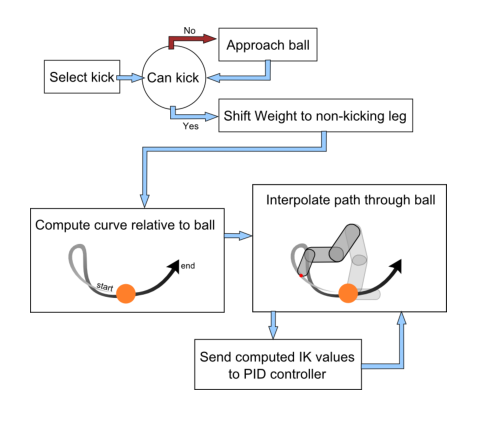
\includegraphics[scale=1]{./data/kick_arch_austin_villa}
	\caption{Schéma vykonania kopu UT Austin Villa \cite{villa2012}}
	\label{pic_kick_arch_austin_villa}
\end{figure}

Použili kubické Hermitove krivky na dosiahnutie dynamického určenia trajektórie nohy vysokou rýchlosťou od pozície lopty. Tieto krivky sa počítajú okamžite, ak vzdialenosť robota od lopty je natoľko dostatočná, aby sa mohol kop vykonať bez ohľadu na to, či je správne natočený. Dokážu dosiahnuť kopy do viacerých smerov. 


%
% tim FC Portugal
%
\subsubsection{FC Portugal} \label{fc_portugal}

Portugalský tím FC Portugal\cite{fc_portugal}, ktorý navrhol metódu pre kopanie do viacerých smerov. Je zložený z troch častí. 

Prvou je vytvorenie dráhy, akou musí smerovať noha robota, aby sa lopta dostala do želaného smeru. Na vytvorenie krivky pohybu nohy použili Bezierovu rovnicu tretieho stupňa. 

Druhou časťou je modul pre inverznú kinematiku, ktorý na základe predtým vypočítanej krivky vypočíta natočenie kĺbov pre vykonanie kopu. 

Posledná časť je stabilizačný modul, ktorý sa snaží dosiahnuť to, aby sa ťažisko robota nachádzalo v ploche druhej podpornej nohy. Do fázy stabilizovania vstupujú aj horné končatiny, ktoré sa upažia alebo predpažia. V extrémnom prípade, ak nestačí pohybovanie rukou, upravuje sa pozícia bokov, členkov a robot sa predkláňa na vyrovnanie stability. Avšak kop nie je dostatočne stabilný. Neriešili parametrizovanie vzdialenosti pri kope.
%Vo výsledkoch boli úspešní pri vypočítavaní krivky (jednoduchý matematický výpočet). Taktiež výsledky dosiahli, že robot kopol loptu do požadovaného smeru. Očakávania nenaplnili pri dosahovaní stability kopu. Neriešili parametrizovanie vzdialenosti.

\begin{figure}[H]
	\center
	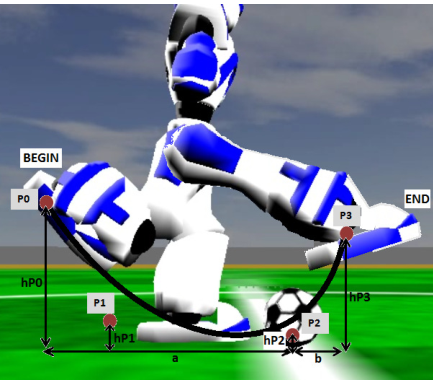
\includegraphics[scale=1]{./data/kick_arch_fc_portugal}
	\caption{Schéma kopu tímu FC Portugal \cite{fc_portugal}}
	\label{pic_kick_arch_fc_portugal}
\end{figure}


\begin{algorithm}
	\caption{Implementácia všesmerového kopu FC Portugal}\label{} 
	\begin{algorithmic}
		\STATE \texttt{foot = chooseFoot()}
		\STATE \texttt{P0, P1, P2, P3 = computeBezierParamters(ball, target, a, b)}
		\FOR {\texttt{i := 1} \TO \texttt{nTrajPoints}}
			\STATE \texttt{trajPoint = computeCurvePoint(P0, P1, P2, P3, nTrajPoints)}
			\STATE \texttt{H = determineRotTransMatrix(trajPoint)}
			\STATE \texttt{joints = computeInverseKinematics(H, foot)}
			\STATE \texttt{joints = computeStability(joints)}
			\STATE \texttt{slots = addSlot(joints, duration)}
		\ENDFOR
		\STATE \texttt{performMovement(slots)}
	\end{algorithmic}
\end{algorithm}

Pohyb začína výberom nohy, ktorou sa bude kopať. Pre výber nohy sa berie do úvahy vzdialenosť od lopty. Pokračuje sa určením parametrov pre Bezierovu krivku, ktorá bude vyjadrovať dráhu pre nohu. Kde vstupné hodnoty do kubickej rovnice Bezierovej krivky pre 4 kontrolné body (\ref{eq_bezier}) vyjadruje obrázok \ref{pic_kick_arch_fc_portugal_params}, kde $t \in [0,1]$.
\begin{equation}\label{eq_bezier}
	b(t) = \sum_{i = 0}^{3}
	{
		{3 \choose i} t^i {(1 - t)}^{3 - i} P_i
	}
\end{equation}

\begin{figure}[H]
	\center
	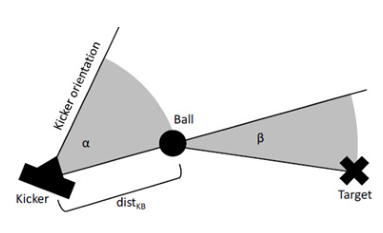
\includegraphics[scale=1]{./data/kick_arch_fc_portugal_params}
	\caption{Parametre potrebné pre výpočet kontrolných bodov krivky všesmerového kopu \cite{fc_portugal}}
	\label{pic_kick_arch_fc_portugal_params}
\end{figure}

Medzi vstupné parametre patrí pozícia lopty a cieľa a tiež uhol medzi vektorom vyjadrujúcim smer natočenia hráča a vektorom spájajúcim pozíciu hráča a pozíciu lopty a nakoniec uhol medzi vektorom hráčovej nohy a lopty a vektorom od lopty k cieľu. Krivka je potom rozdelená na $n$ bodov. Platí nasledovné

\begin{itemize}
 \item sa vypočíta pozícia v priestore
 \item určí sa homogénna matica, ktorá obsahuje natočenia a pozíciu nohy vzhľadom na panvu
 \item vypočítajú sa natočenia pre kĺby pomocou inverznej kinematiky
 \item upravia sa hodnoty kĺbov kvôli stabilizovaniu robota
\end{itemize}
Každý takýto výpočet zodpovedá jednej fáze pohybu. Nakoniec sa vykoná pohyb zo všetkých vypočítaných fáz.

%
% Nao Team Humboldt
%
\subsubsection{Nao Team Humboldt} \label{humboldt}
Tím z berlínskej Humboldtovej univerzity sa venuje aj prispôsobovaniu pohybov na základe podmienok počas hry. V práci \cite{humboldt} sa zamerali na vytvorenie dynamicky prispôsobovanému kopu.

Ich kop pozostáva z 3 aspektov - dosiahnuteľný priestor, naplánovanie pohybu a stabilizovanie. Pohyb je modelovaný v karteziánskom priestore a natočenie kĺbov počítajú na základe inverznej kinematiky. Aby predišli riešeniu zložitého optimalizačného problému, rozhodli sa, že každá nová pozícia kĺbov sa vypočíta v samostatnom výpočtovom cykle.

Plánovanie pohybu kopu si rozdelili na 4 fázy - príprava na kop, odtiahnutie nohy, vykonanie kopu a prinoženie. Počas prípravnej fázy robot nastaví telo tak, aby stál na jednej nohe a nadvihol druhú. Pri odťahovaní nohy si určili funkciu, pri ktorej sa berie do úvahy bod, ktorý je potrebné dosiahnuť, aby nastal zásah do lopty a vektor, ktorý zodpovedá želanému smeru kopu. Výpočet tohto bodu zjednodušili na dvojrozmerný prípad. Súradnicu $z$, ktorá predstavuje výšku chodidla, určili ako konštantu, ktorou je priemer veľkosti lopty. Ak majú určený najlepší bod odtiahnutia, následne sa vykoná pohyb. Dráhu pohybu opisujú veľmi jednoduchým spôsobom. Trajektória predstavuje najkratšiu cestu v priestore medzi bodom odtiahnutia a loptou. Nejde však o najrýchlejší pohyb. Ale rozhodli sa tak preto, lebo pri najrýchlejšom pohybe môže nastať kontakt so zemou. Po odkopnutí lopty sa robot vráti do pôvodnej pozície pred kopom - štvrtá fáza. Ak by sa podmienky počas vykonávania zmenili natoľko, že nie je možné dokončiť kop, robot preruší plánovanie a pokračuje fázou prinoženia do začiatočnej pozície.

Dosiahnuteľný priestor zodpovedá priestoru, ktorý je možné dosiahnuť kopajúcou nohou, zatiaľ čo robot stojí stabilne na druhej nohe. Problém si zjednodušili tak, že nebrali do úvahy natáčanie kĺbov na hraniciach priestoru. Takto im vznikla len trojrozmerná mriežka bez oblúkov. Tento priestor si vypočítali experimentálne na fyzickom robotovi Nao.

Stabilitu vyrovnávajú počas celého pohybu. Pri naplánovaní kopu sú dané pozície oboh nôh. Aby bol robot stabilný, nakláňajú telo robota, aby jeho ťažisko ostalo v podpornom mnohouholníku okolo robota.

%
% praca na univerzite Brémy
%
\subsubsection{Kop v štandardnej lige robotov}\label{sec_bremen}
V tejto časti popíšeme prístupy vykonávania kopov robotov, ktoré boli vytvorené mimo simulovanej 3D ligy. Predlohou simulovanej ligy je robot, ktorý je primárne určený pre štandardnú ligu. Pričom princípy prostredia a pohyby robota sú podobné. 

V práci \cite{bremen} opisujú spôsob, ako vykonávať dynamický kop. Dynamické vykonanie kopu do lopty vychádzalo zo starších prístupov na dynamickú chôdzu. Na výpočet dráhy končatiny opäť použili Bezierove krivky tretieho stupňa. Avšak tentoraz je ich pohyb založený na sekvencii týchto kriviek za sebou. Konkrétne fáza kopu je rozdelená na 7 častí - pristavenie robota k lopte, nadvihnutie chodila, náprah, kopnutie do lopty, nastavenie nohy na pôvodné miesto, spustenie chodidla k zemi a vyrovnanie kĺbov na pôvodné pozície. Schému kopu zobrazuje obrázok \ref{pic_kick_arch_bremen}. 

Krivky pohybu sú vypočítané na základe vstupných parametrov pre kop. Parametrami sú pozícia pre umiestnenie lopty, smer pohybu, číslo fázy a názov končatiny. Z opísaných častí pohybu je možné počas vykonávania meniť náprah a kopnutie do lopty, ktoré sa vie prispôsobiť na základe situácie v čase vykonávania kopu.

Pohyb sa skladá z viacerých pospájaných kriviek v určitých bodov. To má svoju nevýhodu, že ak sú takéto krivky pospájané nedávajú spojitú krivku. Výsledná krivka by mala byť vytvorená tak, aby pohyb bol plynulý bez nejakého prerušenia alebo zaseknutia. 

\begin{figure}[H]
	\center
	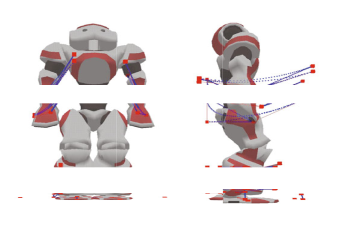
\includegraphics[scale=1]{./data/kick_arch_bremen}
	\caption{Vizualizácia kopu \cite{bremen}}
	\label{pic_kick_arch_bremen}
\end{figure}

Spojiť viac kriviek v spoločnom bode je jednoduchá záležitosť. Avšak takáto krivka nie je derivovateľná vo všetkých bodoch. Deriváciu nemá definovanú práve v spoločnom bode. V článku uvádzajú aj spôsob, za ktorých podmienok je možné dosiahnuť spojitú funkciu. V simulovanej lige nie je potrebné dodržiavať podmienky derivovateľnosti spojených kriviek, pretože pohyby robota prebiehajú vo fázach.

Stabilitu dosiahli implementovali ako samostatný modul. Pre stabilizovanie robota pri kope využili jeho ťažisko. Ťažisko smeruje vždy do zeme a jeho pozíciu umiestňujú do stredu vyvažovacieho mnohouholníka. Mnohouholník má pri kope tvar a veľkosť podpornej nohy. Výpočet je realizovaný ako harmonický priemer $n$ budúcich pozícií podpornej nohy. Vstupom do efektora, ktorý vyrovnáva náklon je rozdiel medzi aktuálnym a vypočítaným bodom ťažiska.

Ostatné externé vplyvy kompenzujú uhlovou rýchlosťou pomocou informácií z gyroskopu. % ... \textit{doplniť}

% co sa nezmestilo a este neviem, kam to dam
%\newpage
%\section{Aktuálny stav} \label{sec_current}

V tejto kapitole uvedieme poznatky, ktoré sme získali po inštalovaní a spúštaní posledne dostupnej verzie robota. Rozhodli sme sa zvoliť dokončenú verziu tímu A55Kickers\footnote{\url{http://labss2.fiit.stuba.sk/TeamProject/2012/team15is-si/dokumenty/agent_robocup_fiit_v2.zip}} (\ref{A55Kickers}) %z mája 2013, pretože v čase dokončovania tejto práce\footnote{máj 2014}, prebieha vývoj v dvoch tímoch na predmete Tímový projekt - Megatroll\footnote{\url{http://labss2.fiit.stuba.sk/TeamProject/2013/team04is-si/}} a Gitmen\footnote{\url{http://labss2.fiit.stuba.sk/TeamProject/2013/team09is-si/}}. 
Postupovali sme podľa návodu na wiki\footnote{\url{http://labss2.fiit.stuba.sk/TeamProject/2013/team09is-si/wiki/index.php/Návody_a_inštalácie}}. Návod bol zrozumiteľný a pri inštalácií potrebného softvéru nenastali žiadne problémy.

Väčšinou sa pre vykonanie kopu používajú staticky definované hodnoty, ktoré sa nachádzajú v XML súbore pre pohyby. Vytváranie nového pohybu je pracné a je potrebné veľké úsilie, aby spĺňal aspoň základné vlastnosti - rýchlosť a hlavne stabilita. Aktuálne pohyby sú spracované na veľmi dobrej úrovni, optimalizované (kapitola \ref{sec_passakp}) a myslíme si, že nie je potrebné vytvárať nové.

Avšak kopy sú rovnaké a navyše kop pri inom nastavení tela hráča, ako je pozícia lopty oproti želanému smeru kopu, si vyžaduje aj prípravnú fázu, počas ktorej sa musí robot postaviť na správne miesto. Zároveň prípravná fáza zaberá dôležitý čas, počas ktorého môže súper sa dostať do vhodnejšej pozície k lopte, prípadne zablokovať strelu.

\subsection{Cieľ}

V tejto práci sme sa rozhodli implementovať parametrizovateľný a dynamický kop. Cieľom vytvorenia tohto kopu je odstrániť už spomínané nedostatky, ktoré boli spomenuté pri realizácii statického kopu. Tento kop by mal byť schopný prispôsobiť sa situácii na ihrisku a umožniť čo najpresnejšie umiestnenie lopty na požadované miesto.

Opísané svetové tímy (kapitoly \ref{austin_villa}, \ref{fc_portugal}, \ref{humboldt}, \ref{sec_bremen}) používajú okrem staticky definovaných pohybov aj pohyby dynamické. 

Aby bolo možné takýto kop používať, je potrebné implementovať taký pohyb, pri ktorom by sa za behu vypočítalo natočenie kĺbov robota. Následne by sa pohyb vykonal. Jedným zo spôsobov je použitie algoritmu portugalského tímu FC Portugal, ktorého všeobecný opis sa nachádza v kapitole \ref{fc_portugal}.

\subsubsection{Inverzná kinematika}

Inverznou kinematikou sa nazýva spôsob výpočtu umiestenia končatiny na vopred stanovenú pozíciu. Vzhľadom na to, že sa dynamickými kopmi nezaoberala žiadna práca na fakulte, je potrebné takýto modul vytvoriť. Ideálne modul, ktorý by bol použiteľný aj pre prípadné ďalšie dynamické pohyby. 

V práci Jána Hudeca\cite{hudec} je navrhnutý spôsob, ako vyriešiť tento problém. Použil by sa čiastočný prístup cez XML súbory, pričom panvové a stehenné kĺby by boli ovládané triedou \texttt{WalkControler}. Trieda by preberala údaje z \texttt{AgentModel}. \texttt{WalkControler} by si stanovil súradnice $[X,Y]$ pre pohyb a na základe nich pohne panvovými a stehennými kĺbmi. V plánovači by sa doplnil pohyb z XML súboru o pozície ostatných kĺbov nôh, príp. rúk. Obrázok \ref{pic_hudec_pohyb_activity_diag} zobrazuje diagram aktivít pre takýto prístup.

\begin{figure}[H]
	\center
	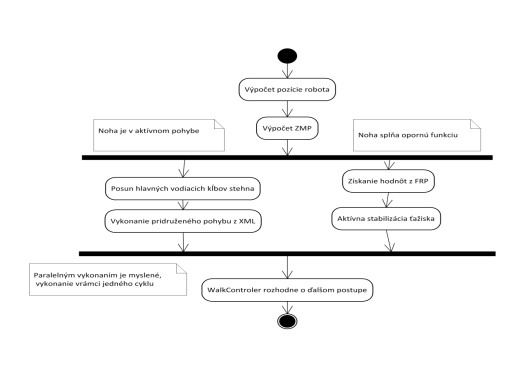
\includegraphics[scale=1]{./data/hudec_pohyb_activity_diag}
	\caption{Aktivity diagram pohybu\cite{hudec}}
	\label{pic_hudec_pohyb_activity_diag}
\end{figure}

Pre pohyb, ktorý by mal byť len dynamický je potrebné upraviť prístup Jána Hudeca a vytvoriť taký modul pre inverznú kinematiku, ktorý by dokázal určiť natočenia kĺbov pre všetky fázy pohybu bez použitia XML súborov.
 
\subsubsection{Stabilita}
%Základom každého pohybu je stabilita hráča. Každý pád môže spôsobiť aj malú časovú stratu, namiesto ktorej by sa mohol venovať hre a pokračovať vo vykonávaní svojho plánu. Ako už bolo spomenuté, pohyby sú dobré spracované a majú aj dostatočnú stabilitu. Pri vytvorení nového dynamicky meniaceho sa kopu je udržanie stability veľká výzva.
%\\
Pre statické hodnoty pohybov z XML súborov platí, že stabilita je riešená tak, že po dokončení pohybu sa musia kĺby natočiť do takej polohy, aby sa predišlo pádom. Tento prístup je pre dynamicky sa meniaci kop nevhodný.

Jedným z výsledkov diplomovej práce Jána Hudeca\cite{hudec} (kap. \ref{sec_auder_hudec}), ktorý je implementovaný vo fakultnom hráčovi JIM je použitie ZMP pre stabilizovanie chôdze.  
%toto mám priamo prebraté z Hudeca
ZMP vyjadruje, že hráč sa nachádza v zóne stability, pokiaľ kolmica na plochu zeme prechádzajúca ťažiskom robota sa nachádza v oblasti opísanej chodidlom v prípade, že hráč stojí na jednej nohe, alebo medzi oboma chodidlami, ak robot stojí na oboch nohách súčasne. ZMP počíta aj s pôsobením ostatných síl na robota - dynamika pohybu, odstredivé sily alebo gravitačná sila.

Rovnice predstavujú vzťahy pre súradnice bodu $ZMP(X_{ZMP}, Y_{ZMP}, 0)$
\begin{equation}
	X_{ZMP} = \frac{\sum_{i=1}^{n}{m_i(\ddot{Z_i} + g_z)X_i - \sum_{i=1}^{n}{m_i(\ddot{X_i} + g_x)Z_i}}}
	{\sum_{i=1}^{n}{m_i(\ddot{Z_i} + g_z)}}
\end{equation}

\begin{equation}
	Y_{ZMP} = \frac{\sum_{i=1}^{n}{m_i(\ddot{Z_i} + g_z)X_i - \sum_{i=1}^{n}{m_i(\ddot{Y_i} + g_y)Z_i}}}
	{\sum_{i=1}^{n}{m_i(\ddot{Z_i} + g_z)}}
\end{equation}

\begin{itemize}
	\item $m_i$ je hmotnosť časti tela $i$, ktorej ťažisko sa nachádza v bode $(X_i, Y_i, Z_i)$ v absolútnom karteziánskom priestore
	\item $g$ je gravitačné zrýchlenie
	\item $\ddot{X_i}$ je druhá derivácia polohy na základe času, teda zrýchlenie v danom bode
\end{itemize}

Hlavná časť implementácie sa nachádza v triede \texttt{AgentModel}, ktorá obsahuje tiež výpočty hybnosti, ťažiska, a výstupy z Force Resistance perceptora.% Ďalšou triedou je \texttt{Joint}, v ktorej sú pokročilé údaje o kĺboch.

%Pri implementácii výslednej verzie hráča som sa rozhodol použiť druhú verziu rovnice na výpočet ZMP z kapitoly 2.5.1 Zero-moment point (začiatok na strane 19) a spresniť ju pomocou hodnôt FR perceptora (ďalej len FRP – viac slovník). Na stabilizáciu využívam hodnoty oboch funkcií súčasne, na spresnenie informácii o hybnosti a pozičnej informácii hráča. JimJet je prvý z Nao robotov na našej fakulte používajúci FR perceptor na jeho stabilizáciu. Na výpočet ZMP a prispôsobenie agenta na server som vykonal úpravy a doplnenia hlavne v Java triedach: FixedObject.java – prispôsobenie hráča na nový server 0.6.5, BodyPart.java – trieda zavádzajúca podrobné informácie o modeli hráča („telesnej stavbe“) a zároveň ponúka funkcionalitu na prácu s výpočtami nad danými časťami tela (computeRelativePositionsToCamera, relativePositionToRoot, ...). AgentModel – doplnenie výpočtov hybnosti, ťažiska, ZMP súradníc, doplnenie o výstup z FRP perceptorov. Joint – doplnenie pokročilých údajov o kĺboch, úprava rozsahu efektorov, pridanie funkcionality Podrobnejšie rozobraté triedy a funkcie, ktoré som implementoval a zmeny v modeli, sú popísané v prílohe E Technická dokumentácia.

%\subsubsection{Prihrávka}
%Prihrávka spočíva v tom, že hráč, ktorý momentálne kontroluje loptu, sa rozhodne, že v danej situácii je výhodnejšia prihrávka ako priamy postup alebo strela. Následne si musí prihrávajúci hráč vybrať spoluhráča, ktorému prihrá a odhadnúť silu prihrávky a miesto, kde by mala prihrávka skončiť. Spracovanie prihrávky hráčom, na ktorého prihrávka smeruje by bolo príliš náročné a preto je lepšie vybrať pozíciu pred hráčom, kde ju môže spoluhráč následne prebrať bez nutnosti loptu zastavovať. 

%Riešenie tohto problému sa dá rozložiť na niekoľko čiastkových problémov, ktoré je následne potrebné zvládnuť na dostatočne kvalitnej úrovni, aby prihrávanie malo vôbec zmysel a prinieslo očakávanú výhodu. Prvou dôležitou časťou je už spomínané vyhodnotenie, kedy by k prihrávke malo prísť, ako aj to, kam by mala smerovať. Miesto, kam má prihrávka smerovať, musí byť pred spoluhráčom vo vzdialenosti len o čosi väčšej ako miesto, kde v momente dorazenia prihrávky bude hráč stáť. Z tohto vyplýva nutnosť zvládnuť samotnú prihrávku na takej kvalitnej úrovni, aby hráč s vysokou úspešnosťou dokázal v relatívne krátkom čase vyslať prihrávku, ktorá skončí na mieste, ktoré bude výhodné pre spoluhráča. 

%Prihrávka, ktorá by bola kratšia, dlhšia alebo nepresná, by mohla zvýhodniť súperiaci tím. Tiež je nutné pri prihrávke vyhodnocovať, či súper nedokáže prihrávku zastaviť, alebo či spoluhráč nie je tiesnení súperom a bude mať dostatok času na ďalšiu interakciu s loptou.

%\subsection{Diplomové práce v roku 2014}

\subsubsection{Diplomová práca Jaroslava Gregu}
Zameranie práce Jaroslava Gregu \cite{grega} bolo na nižšie pohyby a prístupy k tvorbe pohybov a stabilizácii. Analyzoval prístupy na tvorbu dynamických pohybov. Jeho cieľom bolo vytvorenie agenta, ktorý bude vykonávať rýchle pohyby a zároveň bude stabilný. 

Optimalizoval pomalé a nestabilné pohyby použitím genetického algoritmu. Zvýšil rýchlosť pohybu \texttt{walk\_fast} na $0,4~m/s$ a zvýšil silu kopu \texttt{kick\_step\_strong} na $7,12~m$.

Na stabilizovanie hráča využil Zero Moment Point (ZMP). Stabilizovanie prebieha v nasledujúcich krokoch:
\begin{itemize}
	\item získanie informácií o aktuálnom natočení kĺbov a aj o ich nasledujúcom natočení
	\item výpočet ZMP pre aktuálne a budúce natočenie kĺbov
	\item ak sa pozícia nachádza mimo oblasti nôh, hráč sa upraví do takej polohy, aby ZMP bolo v oblasti nôh.
\end{itemize}

\subsubsection{Diplomová práca Pavla Meštaníka} \label{sec_mestanik}

Výsledkom práce Pavla Mešťaníka \cite{mestanik} je implementovaný parametrizovaný priamy kop. Dynamicky dokáže určiť silu kopu na základe definovaj želanej cieľovej pozície lopty. 

Pre určenie takejto funkcie skúmal závislosti kĺbov, ktoré sa podieľajú na sile kopu. Odhalil závislosť bedrového kĺbu \texttt{RLE3} (ekvivalentné pre ľavú nohu a kĺb \texttt{LLE3}). Výsledná funkcia nie je spojitá, ale je po častiach lineárne aproximovateľná. 

Parametrizovaný kop vznikol úpravou statického pohybu pre obe nohy \texttt{kick\_right\_normal} resp. \texttt{kick\_left\_normal}. Začiatočné fázy pohybu sú zhodné so spomínanými kopmi. Dynamicky sa na základe funkcie upraví natočenie bedrového kĺbu a pohyb sa dokončí nastavením do stabilizovanej polohy, ktorá ostáva zo súboru so staticky definovanými kopmi.

Pre dynamický kop vznikol balíček v zdrojovom kóde, ktorý upravuje implementáciu vykonávania staticky definovaných pohybov. Po načítaní pohybu nahradí fázy vypočítaným nastavením a vykonanie pohybu sa vykoná rovnakým spôsobom ako kopy zo súborov.

Výsledné kopnutie je spresnosťou na jedno desiatinné miesto.

\subsubsection{Diplomová práca Tomáša Bolečeka}
Diplomová práca Tomáša Bolečeka \cite{bolecek} je jedinou, ktorá sa nezaoberala nižšími schopnosťami hráčov. Podstatou bolo vytvorenie modelu strategickej vrstvy, aby sa hráči správali ako tím a kooperovali medzi sebou. Vychádzal z prác na FIIT pre simulovanú 2D ligu a svetových 3D tímov. 

Jeho model správania bol navrhnutý pre celý tím a zároveň pre konkrétneho hráča. Správanie rozdelil na viac úrovní, aby sa dali upravovať nezávisle od seba:
\begin{itemize}
\item stratégie
\item taktiky
\item formácie
\item subtaktiky
\item roly
\end{itemize}
Zo správania implementoval formácie a roly, ktoré je možné zamieňať. Pri formáciách sa určuje nie len pozícia, ale aj oblasť, v ktorej by sa mali pohybovať hráči na základe priradenej role. Formácia sa mení dynamicky. Prepočet sa vykonáva každé 3 sekundy. Nie je naviazaná na počet hráčov. Roly sa pri spustení prideľujú na základe štandardných pozícií. Počas hry sa na základe vypočítaného stavu môžu meniť pozície. Predpokladom je, že cena výmeny bude nižšia, ako by bolo zotrvanie v aktuálnej formácii. Algoritmus pre prideľovanie rolí:
\begin{enumerate}
\item vytvoria sa všetky možné dvojice hráčov a rolí na ihrisku
\item vypočíta sa vzdialenosť medzi aktuálnou pozíciou hráča a pozíciou vo formácii.
\item vybraná je tá, ktorá dáva najmenšiu hodnotu.
\end{enumerate}
Najbližší hráč je vždy priradený k lopte. A to aj napriek tomu, že má pridelenú rolu. V tomto prípade ju nebude dodržiavať. Priradenú ju pre prípad, pre jednoduchší návrat do formácie v prípade, že je lopte priradený iný hráč.

Formácie a roly sú uložené v XML súboroch. Formát vychádza zo súborov pre pohyby. Základná štruktúra obsahuje meno formácie, meno autora, popis formácie, počet hráčov, mená hráčov a ich pozície, štartovaciu pozíciu hráčov, určenie, či je možné meniť pozíciu, odstup od lopty, index škálovateľnosti pohybu, veľkosť oblasti pozície.
%Nástroj pre vytváranie XML súborov.


%\subsubsection{Diplomová práca Martina Košického}
%Dynamická chôdza.

%\newpage
%\section{Špecifikácia} \label{sec_specification}

V súčasnom stave sa fakultný robot dokáže pohybovať staticky definovanými pohybmi. Sú definované v XML súbore, v ktorom je napísaná sekvencia fáz natočení kĺbov. V podstate ide o doprednú kinematiku.

V doprednej kinematike pre model robota na základe určených uhlov natočení kĺbov vieme vypočítať bod v priestore, v ktorom sa bude nachádzať koncový efektor. Tento bod vieme získať zo stavu, ktorý si implementácia agenta uchováva v každom serverovom cykle.

Avšak aby sme vedeli hýbať končatinami takým spôsobom, že poznáme body priestore, po ktorých sa má hýbať, potrebujeme vedieť určiť také natočenia kĺbov. Ide o opačný problém ako pri doprednej kinematike. Takýto problém  sa nazýva inverzná kinematika. Výpočet inverznej kinematiky chýba v implementácii fakultného robota. Bez nej nebude možné vytvoriť dynamické pohyby a teda aj dynamické kopanie.

Problémom inverznej kinematiky je, že riešenie je doménovo závislé od modelu. Každá iná konfigurácia kĺbov vedie k inému riešeniu. Narozdiel od doprednej kinematiky, ktorá je doménovo nezávislá.

\subsection{Inverzná kinematika}

Výborným podkladom pre inverznú kinematiku je práca \cite{kofinas, kofinas_master}, kde vypočítali analytickým spôsobom doprednú a inverznú kinematiku pre robota v štandardnej lige robotov. Ich riešenie je rozdelené na 5 nezávislých podproblémov - hlava, ľavá resp. pravá ruka, ľavá resp. pravá noha. Na riešenie využili metódu vyjadrenia transformačných matíc pre postupnosti kĺbov pomocou Denavit-Hartenbergových parametrov.

\subsubsection{Analytické riešenie tímu Kouretes}
Vychádzajú zo všeobecnej transformačnej matice v $n$-rozmernom priestore veľkosti $(n+1)\times (n+1)$, ktorá má nasledujúci tvar:
\begin{equation}
	T = \left[
	\begin{tabular}{cc}
		X & Y \\
		$[0\ldots0]$ & 1
	\end{tabular}
	\right]
\end{equation}
kde $X$ je matica rozmerov $(n\times n)$, $Y$ je vektor $(n \times 1)$.
\\

Ďalej traslačná matica, ktorá vyjadruje posun bodu v priestore o pevnú vzdialenosť má tvar:
\begin{equation}
	T = \left[
	\begin{tabular}{cc}
		I & 
			\begin{tabular}{c}
				$d_x$ \\
				$d_y$ \\
				$d_z$
			\end{tabular}
			 \\
		$[0\ldots0]$ & 1
	\end{tabular}
	\right]
\end{equation}
kde $d_x$, $d_y$, $d_z$ vyjadrujú vzdialenosť posunu po osiach $x$, $y$ a $z$. Ide vlastne o transformačnú maticu $X=I$.
\\

Rotačná matica vyjadruje otočenie  vektora o určený uhol v trojrozmernom priestore. Existujú 3 rôzne matice, každá vyjadruje otočenie okolo jednej osi.
\begin{align}
	R_x &= \left[
	\begin{tabular}{ccc}
	 1 & 0 & 0 \\
	 0 & $\cos\theta_x$ & $-\sin\theta_x$ \\
	 0 & $\sin\theta_x$ & $\cos\theta_x$
	\end{tabular}
	\right]	
		\nonumber \\
		\nonumber \\
	R_y &= \left[
	\begin{tabular}{ccc}
	 $\cos\theta_y$ & 0 & $\sin\theta_y$ \\
	 0 & 1 & 0 \\
	 $-\sin\theta_y$ & 0 & $\cos\theta_y$
	\end{tabular}
	\right] 
		\nonumber \\
		\nonumber \\
	R_z &= \left[
	\begin{tabular}{ccc}
	 $\cos\theta_z$ & $-\sin\theta_z$ & 0 \\
	 $\sin\theta_z$ & $\cos\theta_z$ & 0 \\
	 0 & 0 & 1
	\end{tabular}
	\right]
\end{align}

Kombináciou rotačných matíc okolo zodpovedajúcich osí v priestore a posunu od vzdialenosť $d$ vyjadreného vektorom $d=(d_x, d_y, d_z)^T$ dostaneme transformačnú maticu v trojrozmernom priestore:
\footnotesize
\begin{align}
   T&=\left[
	\begin{tabular}{cc}
		$\hat{R}$ & 
			\begin{tabular}{c}
				$d_x$ \\
				$d_y$ \\
				$d_z$
			\end{tabular} \\
		$[0\ldots0]$ & 1
	\end{tabular}
	\right] = \nonumber \\
	&=\left[
	\begin{tabular}{cccc}
		$\cos a_y \cos a_z$ & $-\cos a_x \sin a_z + \sin a_x \sin a_y \cos a_z$ & $\sin a_x \sin a_z + \cos a_x  \sin a_y \cos a_z$ & $p_x$ \\
		$\cos a_y \sin a_z$ & $\cos a_x \cos a_z + \sin a_x \sin a_y \sin a_z$ & $-\sin a_x \cos a_z + \cos a_x \sin a_y \sin a_z$ & $p_y$ \\
		$-\sin a_y$ & $\sin a_x \cos a_y$ & $\cos a_x \cos a_y$ & $p_z$ \\
		0 & 0 & 0 & 1
	\end{tabular}
	\right]
\end{align}

\normalsize
kde $\hat{R} = R_xR_yR_z$.
\\

Ďalším zo spôsobov vytvorenie transformačnej matice, ktorá vyjadruje bod na jednom konci kĺbu vzhľadom na iný koncový bod kĺbu pomocou 4 parametrov $a$, $\alpha$, $d$ a $\theta$. Tieto parametre sa nazývajú Denavit-Hartenbergove a majú nasledovný význam:
\begin{itemize}
	\item $a$ - normálová vzdialenosť kĺbov
	\item $\alpha$ - uhol pri normále od osi $z_{i-1}$ k osi $z_i$
	\item $d$ - posun od osi $z_{i-1}$ k normále
	\item $\theta$ - uhol okolo osi $z_{i-1}$ smerom od osi $x_{i-1}$ k osi $x_i$
\end{itemize}
$i$ vyjadruje poradie kĺbu.

Výsledná transformačná matica je vyjadrená kombináciou 2 rotačných a 2 translačných matíc pre Denavit-Hartenbergove parametre:
\begin{equation}
	T_{DH} = R_x(\alpha)T_x(a)R_z(\theta)T_z(d) =
	\left[
	\begin{tabular}{cccc}
		$\cos \theta$ & $-\sin \theta$ & $0$ & $a$ \\
		$\sin\theta\cos\alpha$a & $\cos\theta\cos\alpha$ & $-\sin\alpha$ & $-d\sin\alpha$ \\
		$\sin\theta\cos\alpha$ & $\cos\theta\sin\alpha$ & $\cos\alpha$ & $d\cos\alpha$ \\
		$0$ & $0$ & $0$ & $1$
	\end{tabular}
	\right]
\end{equation}

Ako východzia pozícia $[0~0~0]$ bol zvolený bod na trupe robota, ktorý zároveň predstavuje ťažisko. Všetky pozície kĺbov sú počítané relatívne k počiatočnému bodu.
\\\\
Z výslednej transformačnej matice $T$, ktorá vznikne kombinovaním rotačných a posuvných matíc, je možné odvodiť výslednú pozíciu a natočenie koncového vektora pre danú sekvenciu kĺbov.


\begin{equation}
p_x = T_{\left(1,4\right)}
\end{equation}
\begin{equation}
p_y = T_{\left(2,4\right)}
\end{equation}
\begin{equation}
p_z = T_{\left(3,4\right)}
\end{equation}

\begin{equation}
a_x = \arctan2\left(T_{\left(3,2\right)},T_{\left(3,3\right)}\right)
\end{equation}
\begin{equation}
a_y = \arctan2\left(-T_{\left(3,1\right)},\sqrt{T_{\left(3,2\right)}^2 + T_{\left(3,3\right)}^2}\right)
\end{equation}
\begin{equation}
a_z = \arctan2\left(T_{\left(2,1\right)},T_{\left(1,1\right)}\right)
\end{equation}
kde $(p_x, p_y, p_z)$ je pozícia v priestore a $(a_x, a_y, a_z)$ je výsledné natočenie vzhľadom na zodpovedajúce osi.
\\\\
Pre analytické riešenie inverznej kinematiky využili transformačnú maticu. Do tej sa dosadia hodnoty koncovej pozície efektora príslušnej končatiny. Takto vznikne numerické riešenie. Táto matica sa dá do rovnosti so symbolickou transformačnou maticou pre doprednú kinematiku pre každú končatinu, ktorá vznikne vynásobením rotačných a translačných matíc. Tieto rovnice sú uvedené v kapitole \ref{sec_forward_kinematics_equations}.


\subsubsection{Rovnice pre doprednú kinematiku}\label{sec_forward_kinematics_equations}
\noindent
\textbf{Hlava}

\begin{equation}
T_{\text{Base}}^{\text{End}} = A_{\text{Base}}^{0} T_{1}^{2} R_{x}\left(\frac{\pi}{2}\right) R_{y}\left(\frac{\pi}{2}\right) A_{4}^{\text{end}}
\end{equation}

\noindent
\textbf{Ľavá ruka}

\begin{equation}
T_{\text{Base}}^{\text{End}} = A_{\text{Base}}^{0} T_{1}^{2} T_{2}^{3} T_{3}^{4} R_{z}\left(\frac{\pi}{2}\right) A_{4}^{\text{End}}
\end{equation}

\noindent
\textbf{Pravá ruka}

\begin{equation}
T_{\text{Base}}^{\text{End}} = A_{\text{Base}}^{0} T_{1}^{2} T_{2}^{3} T_{3}^{4} R_{z}\left(\frac{\pi}{2}\right) A_{4}^{\text{End}} R_{z}\left(\pi\right)
\end{equation}

\noindent
\textbf{Ľavá noha}

\begin{equation}
T_{\text{Base}}^{\text{End}} = A_{\text{Base}}^{0} T_{1}^{2} T_{2}^{3} T_{3}^{4} T_{4}^{5} T_{5}^{6} R_{z}\left(\pi\right) R_{y}\left(\frac{\pi}{2}\right) A_{6}^{\text{End}}
\end{equation}

\noindent
\textbf{Pravá noha}

\begin{equation}
T_{\text{Base}}^{\text{End}} = A_{\text{Base}}^{0} T_{1}^{2} T_{2}^{3} T_{3}^{4} T_{4}^{5} T_{5}^{6} R_{z}\left(\pi\right) R_{y}\left(\frac{\pi}{2}\right) A_{6}^{\text{End}} 
\end{equation}

Kde $T_{\text{Base}}^{\text{End}}$ je výsledná transformačná matica od počiatočného kĺbu ku koncovému kĺbu. $A_{\text{Base}}^{0}$ vyjadruje posunutie počiatočného kĺbu pre príslušnú končatinu vzhľadom k trupu, $T_{i}^{j}$ je transformácia medzi kĺbami $i$ a $j$ v postupnosti, $R_x$ resp. $R_y$, $R_z$ rotácia kĺbu o uhol $\theta$ a $A_{n}^{\text{End}}$ posun koncového efektora oproti $n$-tému kĺbu končatiny.

%\newpage
%\subsubsection{Rovnice pre inverznú kinematiku} \label{sec_inverse_kinematics_equations}
\textbf{Ľavá ruka}\\
Ľavá ruka sa skladá zo 4 kĺbov, pre ktoré sa vypočítajú uhly $\theta_1$, $\theta_2$, $\theta_3$, $\theta_4$.
\begin{equation}
	\theta_4 = -\left(\pi - \arccos\left(\frac{l_3^2 + l_4^2 - \sqrt{\left(s_x - T_{\left(1,4\right)}\right)^2 + \left(s_y - T_{\left(2,4\right)}\right)^2 + \left(s_z - T_{\left(3,4\right)}\right)^2}^2}{2l_3l_4}\right)\right)
\end{equation}

\begin{equation}
	\theta_2 = \pm \arccos{\left(\frac{T_{\left(2,4\right)}-l_1-\left(\frac{l_4 \sin{\theta_4}T_{\left(2,2\right)}}{\cos{\theta_4}}\right)}{l_3 + l_4\cos{\theta_4}+l_4\frac{\sin^2{\theta_4}}{\cos{\theta_4}}}\right)} + \frac{\pi}{2}
\end{equation}

\begin{equation}
	\begin{tabular}{c}
		$\theta_3 = -\arcsin\left(\frac{T_{\left(2,3\right)}}{\sin\left(\theta_2 - \frac{\pi}{2}\right)}\right)$ \\\\
		$\theta_3 = -\left(\pi - \arcsin\left(\frac{T_{\left(2,3\right)}}{\sin\left(\theta_2 - \frac{\pi}{2}\right)}\right)\right)$
	\end{tabular}
\end{equation}

\begin{equation}
	\begin{tabular}{lr}
		$\theta_1=\pm \arccos\left(\frac{T_{\left(3,3\right)} + \frac{T_{\left(1,3\right)}\sin\left(-\theta_3\right)\cos\left(\theta_2 - \frac{\pi}{2}\right)}{\cos\left(-\theta_3\right)}}{\cos\left(-\theta_3\right) + \frac{\cos^2\left(\theta_2 - \frac{\pi}{2}\right) \sin^2\left(-\theta_3\right)}{\cos\left(-\theta_3\right)}}\right)$ & 
	$\text{if }\theta_3 \neq \left|\frac{\pi}{2}\right|$
	\end{tabular}
\end{equation}

% mozno upravit pomocou tabulky, alebo zistit, ako zvacsit pismo
\begin{equation}
	\theta_1 = \pm \arccos\left(\frac{T_{\left(1,3\right)}}{\cos\left(\theta_2 - \frac{\pi}{2}\right) \sin\left(-\theta_3\right)}\right)
	\text{if }\theta_3 = \left|\frac{\pi}{2}\right|\text{ and }\theta_2 \neq 0
\end{equation}

$$\widehat{T} = T\left(A_4^{End}\right)^{-1}$$

\begin{equation}
	\theta_1 = \pm \arccos\left(\frac{\widehat{T}_{\left(1,4\right)}}{l_3}\right)
	\text{if }\theta_3 = \left|\frac{\pi}{2}\right|\text{ and }\theta_2 = 0
\end{equation}
\\\\
\textbf{Pravá ruka}\\
	Rovnica pre riešenie uhlov $\theta_1$, $\theta_2$, $\theta_3$, $\theta_4$ sa pre pravú ruku líši oproti ľavej ruke v hodnotách Denavit-Hartenberg parametrov a fixácii rotácie začiatočného kĺbu $R_x(\pi)$, ktorá sa vykráti z oboch strán rovnice. Riešenie je uvedené v \cite{kofinas_master}.
\\\\
\textbf{Ľavá noha}
\\Ľavá noha sa skladá zo 6 kĺbov, pre ktoré sa vypočítajú uhly $\theta_1$, $\theta_2$, $\theta_3$, $\theta_4$, $\theta_5$, $\theta_6$.

$$T'=\left(R_x\left(\frac{\pi}{4}\right) \left(\left(A_{Base}^0\right)^{-1}T\left(A_6^{End}\right)^{-1} \right) \right)^{-1}$$
\begin{equation}
	\theta_4 = \pm \left(\pi - \arccos\left(\frac{l_1^2 + l_2^2 - \sqrt{\left(0-T'_{\left(1,4\right)}\right)^2 + \left(0-T'_{\left(2,4\right)}\right)^2 + \left(0-T'_{\left(3,4\right)}\right)^2}^2 }{2l_1l_2}\right)\right)
\end{equation}

\begin{equation}
	\theta_6 = \arctan\left(\frac{T'_{\left(2,4\right)}}{T'_{\left(3,4\right)}}\right)
	\text{if }\left(l_2\cos\theta_5 + l_1\cos\left(\theta_4 + \theta_5\right)\right) \neq 0
\end{equation}

\begin{equation}
	\theta_6 = 0
	\text{if }\left(l_2\cos\theta_5 + l_1\cos\left(\theta_4 + \theta_5\right)\right) = 0 
\end{equation}

$$T''=\left(\left(T'\right)^{-1} \left(T_5^6 R_z\left(\pi\right) R_y\left(-\frac{\pi}{2}\right)\right)^{-1}\right)^{-1}$$

\begin{equation}
	\theta_5 = \arcsin\left(-\frac{T''_{\left(2,4\right)} \left(l_2 + l_1\cos\theta_4\right) + l_1T''_{\left(1,4\right)}\sin\theta_4 } {l_1^2\sin^2 \theta_4 + \left(l_2 + l_1\cos\theta_4\right) }\right)
\end{equation}

\begin{equation}
	\theta_5 = \pi - \arcsin\left(-\frac{T''_{\left(2,4\right)} \left(l_2 + l_1\cos\theta_4\right) + l_1T''_{\left(1,4\right)}\sin\theta_4 } {l_1^2\sin^2 \theta_4 + \left(l_2 + l_1\cos\theta_4\right) }\right)
\end{equation}

$$T''' = \left(T''\right)^{-1} \left(T_3^4 T_4^5\right)^{-1}$$

\begin{equation}
	\theta_2 = \pm \arccos\left(T'''_{\left(2,3\right)}\right) + \frac{\pi}{4}
\end{equation}

\begin{equation}
	\theta_3 = \arcsin\left(\frac{T'''_{\left(2,2\right)}}{\sin\left(\theta_2 + \frac{\pi}{4}\right)}\right)
\end{equation}

\begin{equation}
	\theta_3 = \pi - \arcsin\left(\frac{T'''_{\left(2,2\right)}}{\sin\left(\theta_2 + \frac{\pi}{4}\right)}\right)
\end{equation}

\begin{equation}
	\theta_1 = \pm \arccos\left(\frac{T'''_{\left(1,3\right)}}{\sin\left(\theta_2 + \frac{\pi}{4}\right)}\right) + \frac{\pi}{2}
\end{equation}
\\\\
\textbf{Pravá noha} \\
Riešenie sa líši v transformačných maticiach Denavit-Hartenbergových parametrov a je uvedené v \cite{kofinas_master}.
\\

Z práce využijeme výsledné rovnice uhlov pre všetky končatiny. Analytické riešenie v príslušnom zdroji \cite{kofinas, kofinas_master}.

Oproti použitému riešeniu zo štandardnej ligy sa model robota v simulovanej lige líši. Ide len o rozmery končatín a kĺbov. Ide o konštanty, na ktorých je analytické riešenie nezávislé. Všetky konštanty nájdeme v prílohe  \ref{appendix_nao_model}.
%\newpage
%\section{Implementácia}

Aby fakultný robot dokázal využívať pohyby vypočítané inverznou kinematikou, opísané v kapitole \ref{sec_specification}, rozhodli sme sa výpočet, čo najviac oddeliť od súčasnej štruktúry kódu. Ako podklad sme si zvolili implementáciu diplomovej práce Pavla Meštaníka, ktorá je opísaná v kapitole \ref{sec_mestanik}. Vznikol tak samostatný balíček v jazyku Java s menom \texttt{sk.fiit.jim.agent.moves.ik}. 

Súčasťou sú tieto triedy:
\begin{itemize}
	\item \texttt{ForwardKinematicResult}
	\item \texttt{HeadIk}
	\item \texttt{Kinematics}
	\item \texttt{KinematicUtils}
	\item \texttt{LeftArmIk}
	\item \texttt{LeftLegIk}
	\item \texttt{Matrix}
	\item \texttt{Orientation}
	\item \texttt{RightArmIk}
	\item \texttt{RightLegIk}
	\item \texttt{SimsparkConstants}
\end{itemize}

Triedy \texttt{Kinematics}, \texttt{Matrix}, \texttt{Orientation} sú jediné, ktoré sú viditeľné aj v iných balíčkoch, ostatné sú viditeľné len v rámci nového balíka. V nasledujúcej kapitole \ref{sec_classes_desc} si popíšeme funkcionalitu každej triedy.

\subsection{Popis tried} \label{sec_classes_desc}
\textbf{Trieda \texttt{Kinematics}}
\\
Táto trieda obsahuje metódy, ktoré slúžia na vrátenie výsledkov výpočtov pre doprednú a inverznú kinematiku popísaných rovnicami z kapitoly \ref{sec_specification} pre všetky 4 končatiny (ľavú, resp. pravú ruku a ľavú, resp. pravú ruku). Výpočet pre hlavu sa momentálne nevyužíva.
\\\\
\textbf{Trieda \texttt{Matrix}}
\\
Slúži sa na maticové operácie, ktoré sa využívajú pri doprednej a inverznej kinematike. Zároveň obsahuje niektoré matice ako konštanty, ktoré sa často využívajú pri výpočtoch. 
\\\\
\textbf{Trieda \texttt{Orientation}}
\\
Úlohou tejto triedy je zapuzdriť natočenie koncového efektora podľa zodpovedajúcich osí $x$, $y$, $z$.
\\\\
\textbf{Triedy \texttt{LeftArmIk}, \texttt{LeftLegIk}, \texttt{RightArmIk}, \texttt{RightLegIk}, \texttt{HeadIk}}
\\
Obsahujú výpočty pre uhly zodpovedajúcim končatinám.
\\\\
\textbf{Triedy \texttt{SimsparkConstants}, \texttt{KinematicUtils}}
\\
Pomocné triedy na uchovávanie konštánt a pomocných metód pre všetky ostatné výpočty.
\\\\
\textbf{Ostatné triedy}
Zároveň boli rozšírené existujúce balíčky novými triedami. Tie slúžia na využije inverznej kinematike pri pohyboch robota. Nové triedy:
\begin{itemize}
	\item \texttt{DynamicMove} - slúži ako predloha pre dynamické pohyby pre \texttt{Ruby} triedy. Vstupom je sekvencia pozícií a natočení koncového vektora zodpovedajúcej končatiny.
	\item \texttt{RubyDynamicMove} - slúži na vytváranie sekvencií pozícií a natočení koncového efektora niektorej končatiny, teda vytvára pohyb.
	\item \texttt{PlanDynamicMove} - trieda pre plánovač, na využívanie dynamických pohybov.
\end{itemize}

Závislosti medzi triedami a balíčkami sú zobrazené na obrázku \ref{pic_class_diagram}. Obrázok neobsahuje všetky triedy, ale len relevantné pre opis implementácie. Novovytvorené triedy a balíčky sú zvýraznené tmavou farbou.

\begin{landscape}
\thispagestyle{empty}
\newgeometry{right=-8cm} % magické číslo, aby to bolo pekne zarovnané.
\begin{figure}[H]
\centering
	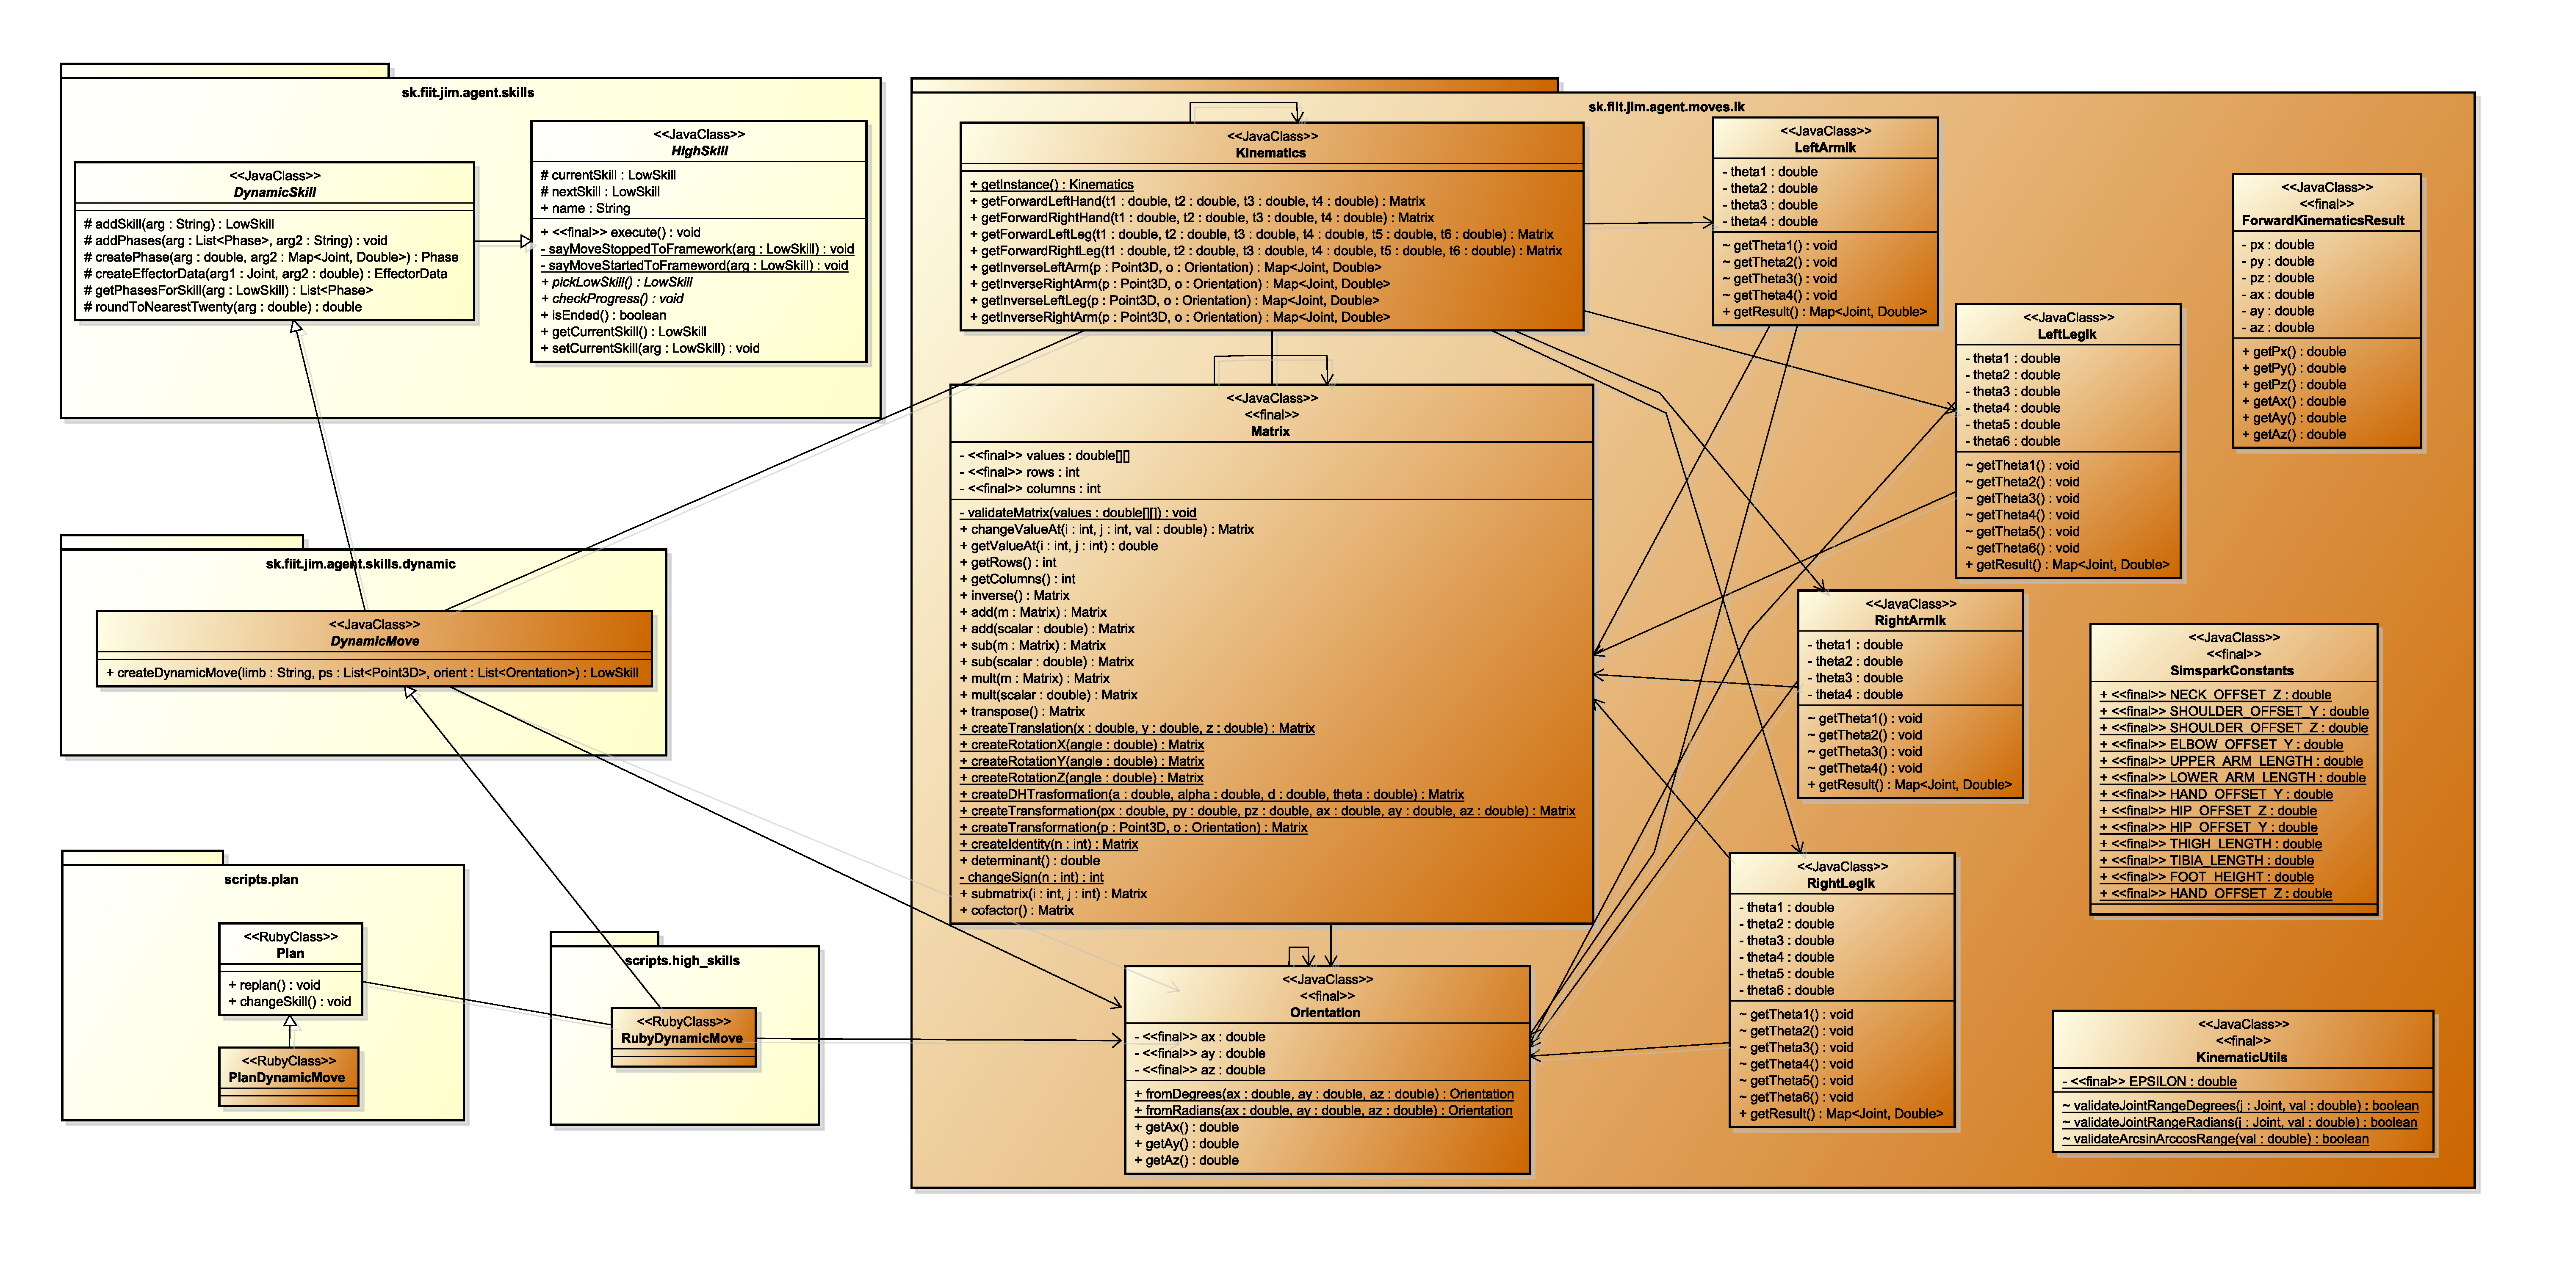
\includegraphics[scale=0.3]{./data/class_diagram}
	\caption{sdnaidna}
	\label{pic_class_diagram}
\end{figure}
\end{landscape}

%\newpage
%\section{Overenie riešenia} \label{sec_verification}

Implementáciu sme sa pokúsili vyskúšať na jednoduchej situácii. Do plánovača sme doplnili novú triedu a súčasne vytvorili nový pohyb, ktorý je vložený do plánovača. Trieda pre pohyb vytvorí sekvenciu koncových bodov a natočení v priestore pre koncový efektor. Tieto sekvencie necháme vykonať na simulačnom prostredí.

Vytvorili sme 2 pohyby - jeden pre ľavú ruku a jeden pre ľavú nohu. Pokus s ľavou nohou sa vykonáva po páde robota. Aktuálna implementácia neberie do úvahy stabilitu robota. Pri pohybe nohou by spadol, aj keby začal vo vzpriamenej polohe. Pokusné body je možné meniť v Ruby triede \texttt{RubyDynamicMove}. Avšak musia byť dosiahnuteľné natočením kĺbov. 

Videá sú dostupné na priloženom médiu (viď príloha \ref{appendix_medium}).

\newpage
\section{Zhodnotenie a ďalšia práca} \label{sec_conclusion}

Na základe analyzovaných riešení sme vytvorili prototyp pre fakultného hráča, ktorý dokáže využiť inverznú kinematiku a vypočítať veľkosti uhlov v končatinách, aby sa efektor dostal na želanú pozíciu. Implementáciu inverznej kinematiky sme sa snažili urobiť čo najviac nezávislú od existujúceho kódu. Vznikol nový Java balíček.

Urobili sme tak základ pre vytvorenie nového spôsobu vytvárania pohybov. To umožní vytvoriť nové pohyby, príp. nahradiť niektoré staticky definované pohyby v XML súboroch novými dynamicky definovanými.

Pohyby robota fungujú. Dokážeme vypočítať natočenie uhlov, aby sa koncový efektor dostal na želanú pozíciu. Pohyby pre dolné končatiny sú momentálne nestabilné. V ďalšej práci je potrebné doplniť vytvorenie pohybu takým spôsobom, aby robot nepadal. Pokúsime sa využiť existujúce riešenia opísané v analýze.

Ďalšou možnosťou je nájsť spôsob, ako zafixovať hodnoty niektorých uhlov tak, aby sa efektor dostal na želanú pozíciu. Momentálne sú výpočty závislé na predošlom výpočte a neexistuje vyjadrenie rovnice hodnoty uhla opačným spôsobom.

Začali sme pracovať s implementáciou od Pavla Meštaníka (kapitola \ref{sec_mestanik}), ktorá ešte využívala Ruby skriptovanie. V súčasnej implementácii fakultného robota, ktorú vyvíjajú na tímových projektoch\footnote{Tím 8 Infinity - v akademickom roku 2014/2015 \url{http://labss2.fiit.stuba.sk/TeamProject/2014/team08is-si/} }, boli odstránené časti kódu v Ruby a plne nahradené Javou. Ďalším cieľom je pripojiť sa k hlavnej vetve vývoja na fakulte k repozitáru tímového projektu a nefragmentovať funkcionalitu. Predpokladáme, že integrácia kódu z tejto diplomovej práce a kódu tímového projektu prebehne bez väčších komplikácií, pretože vytvorený prototyp má málo závislosti na iné časti kódu.


\newpage
\bibliographystyle{acm}
%plain, ieeetr, jbact
\bibliography{references}

\newpage
\appendix					% čislovanie kapitol pre prílohy, abecedne
%\section{Model a rozmery robota Nao v simulovanej 3D lige}
	\label{appendix_nao_model}
asdasd
\begin{figure}[H]
  \center
  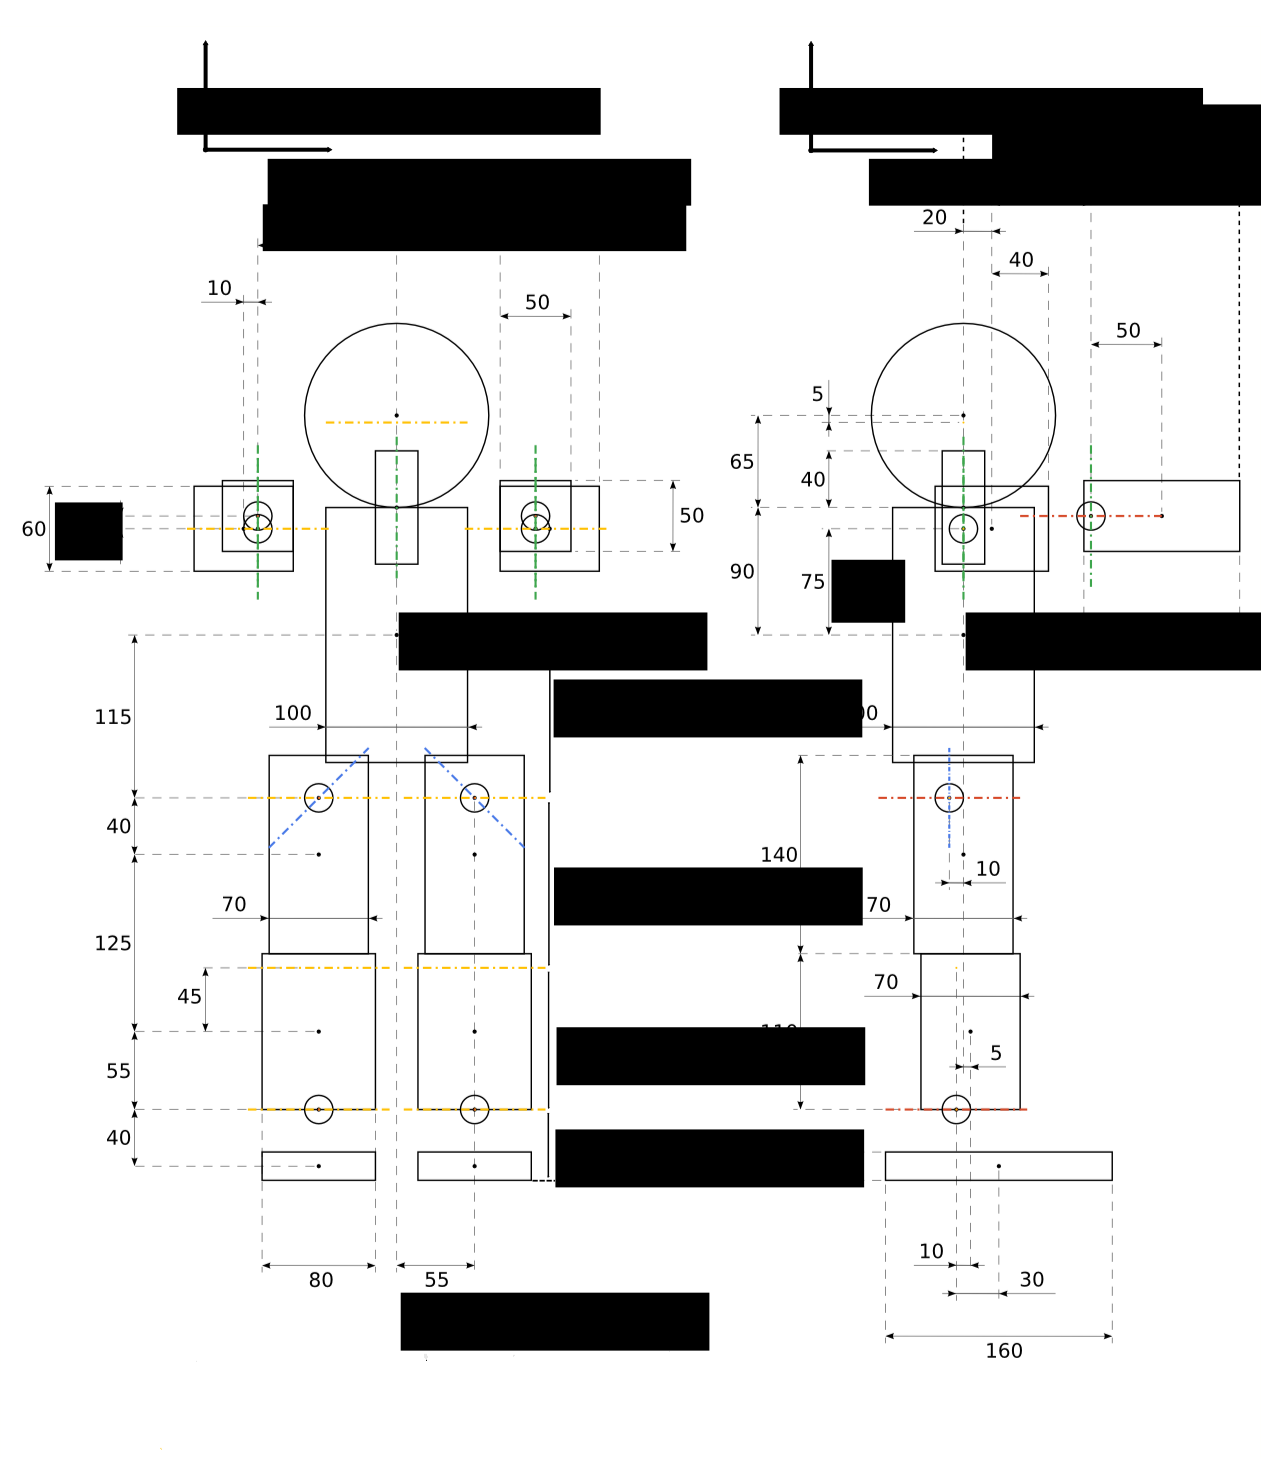
\includegraphics[scale=1.5]{./data/nao_model}
  \caption{Model robota v simulovanej 3D lige \cite{simspark}}
  \label{nao_model}
\end{figure}
\begin{center}
\begin{tabular}{|l|r|}
\hline
\textbf{Končatina} & \textbf{Rozmer (mm)} \\ 
\hline
ShoulderOffsetY	& 98 \\
\hline
ElbowOffsetY & 0 \\
\hline
UpperArmLength & 90 \\
\hline
LowerArmLength & 105 \\
\hline
ShoulderOffsetZ	& 75 \\
\hline
HandOffsetX	& 0 \\
\hline
HandOffsetZ & 9 \\
\hline
HipOffsetZ & 115 \\
\hline
HipOffsetY & 55 \\
\hline
ThighLength	& 120 \\
\hline
TibiaLength	& 100 \\
\hline
FootHeight & 50 \\
\hline
NeckOffsetZ & 90 \\
\hline
\end{tabular}
\end{center}
%\newpage
%\section{Parameter Denavit Hanenberg} \label{appedix_dh}

\subsection{hlava}
\begin{center}
	\begin{tabular}{|l|c|c|c|c|}
	\hline
	\textbf{Kĺb} & $\textbf{a}$ & $\mathbb{\alpha}$ & $\textbf{d}$ & $\theta$ \\
	\hline
	Base & \multicolumn{4}{|c|}{A(0, 0, NeckOffsetZ)} \\
	\hline
	HeadYaw & 0 & 0 & 0 & $\theta_1$ \\
	\hline
	HeadPitch & 0 & $-\frac{\pi}{2}$ & 0 & $\theta_2 - \frac{\pi}{2}$ \\
	\hline
	Rotation & \multicolumn{4}{|c|}{$R_x\left(\frac{\pi}{2}\right)R_y\left(\frac{\pi}{2}\right))$} \\
	\hline
	Top Camera & \multicolumn{4}{|c|}{A(topCameraX, 0, topCameraZ)} \\
	\hline
	Bottom Camera & \multicolumn{4}{|c|}{A(bottomCameraX, 0, bottomCameraZ)} \\
	\hline
	%\multicolumn{1}{|c|}{ \scriptsize{topCameraX=53.9mm, topCameraZ=67.9mm, bottomCameraX=48.8mm, bottomCameraZ=23.8mm}} \\
	%\hline
	\end{tabular}
\end{center}

\subsection{ľavá ruka}
\begin{center}
	\begin{tabular}{|l|c|c|c|c|}
	\hline
	\textbf{Kĺb} & $\textbf{a}$ & $\mathbb{\alpha}$ & $\textbf{d}$ & $\theta$ \\
	\hline
	Base & \multicolumn{4}{|c|}{A(0, ShoulderOffsetY+ElbowOffsetY, ShoulderOffsetZ)} \\
	\hline
	LShoulderPitch & 0 & $-\frac{\pi}{2}$ & 0 & $\theta_1$ \\
	\hline
	LShoulderRoll & 0 & $\frac{\pi}{2}$ & 0 & $\theta_2 - \frac{\pi}{2}$ \\
	\hline
	LElbowYaw & 0 & $-\frac{\pi}{2}$ & UpperArmLength & $-\theta_3$ \\
	\hline
	LElbowRoll & 0 & $\frac{\pi}{2}$ & 0 & $-\theta_4$ \\
	\hline
	Rotation & \multicolumn{4}{|c|}{$R_z\left(\frac{\pi}{2}\right)$} \\
	\hline
	End effector & \multicolumn{4}{|c|}{A(HandOffsetX+LowerArmLength, 0, 0)} \\
	\hline
	\end{tabular}
\end{center}

\subsection{pravá ruka}
\begin{center}
	\begin{tabular}{|l|c|c|c|c|}
	\hline
	\textbf{Kĺb} & $\textbf{a}$ & $\mathbb{\alpha}$ & $\textbf{d}$ & $\theta$ \\
	\hline
	Base & \multicolumn{4}{|c|}{A(0, -ShoulderOffsetY-ElbowOffsetY, ShoulderOffsetZ)} \\
	\hline
	LShoulderPitch & 0 & $-\frac{\pi}{2}$ & 0 & $\theta_1$ \\
	\hline
	LShoulderRoll & 0 & $\frac{\pi}{2}$ & 0 & $\theta_2 + \frac{\pi}{2}$ \\
	\hline
	LElbowYaw & 0 & $-\frac{\pi}{2}$ & -UpperArmLength & $-\theta_3$ \\
	\hline
	LElbowRoll & 0 & $\frac{\pi}{2}$ & 0 & $-\theta_4$ \\
	\hline
	Rotation & \multicolumn{4}{|c|}{$R_z\left(\frac{\pi}{2}\right)$} \\
	\hline
	End effector & \multicolumn{4}{|c|}{A(-HandOffsetX-LowerArmLength, 0, 0)} \\
	\hline
	Rotation fix & \multicolumn{4}{|c|}{$R_z\left(\pi\right)$} \\
	\hline
	\end{tabular}
\end{center}

\subsection{ľavá noha}
\begin{center}
	\begin{tabular}{|l|c|c|c|c|}
	\hline
	\textbf{Kĺb} & $\textbf{a}$ & $\mathbb{\alpha}$ & $\textbf{d}$ & $\theta$ \\
	\hline
	Base & \multicolumn{4}{|c|}{A(0, HipOffsetY, -HipOffsetZ)} \\
	\hline
	LHipYawPitch & 0 & $-\frac{3\pi}{4}$ & 0 & $\theta_1 - \frac{\pi}{2}$ \\
	\hline
	LHipRoll & 0 & $-\frac{\pi}{2}$ & 0 &  $\theta_2 + \frac{\pi}{4}$ \\
	\hline
	LHipPitch & 0 & $\frac{\pi}{2}$ & 0 & $\theta_3$ \\
	\hline
	LKneePitch & -ThighLength & 0 & 0 & $\theta_4$ \\
	\hline 
	LAnklePitch & -TibiaLength & 0 & 0 & $\theta_5$ \\
	\hline
	LAnkleRoll & 0 & $\frac{\pi}{2}$ & 0 & $\theta_5$ \\
	\hline
	Rotation & \multicolumn{4}{|c|}{$R_z\left(\pi\right)R_y\left(-\frac{\pi}{2}\right)$} \\
	\hline
	End effector & \multicolumn{4}{|c|}{A(0, 0, -FootHeight)} \\
	\hline
	\end{tabular}
\end{center}

\subsection{pravá noha}
\begin{center}
	\begin{tabular}{|l|c|c|c|c|}
	\hline
	\textbf{Kĺb} & $\textbf{a}$ & $\mathbb{\alpha}$ & $\textbf{d}$ & $\theta$ \\
	\hline
	Base & \multicolumn{4}{|c|}{A(0, -HipOffsetY, -HipOffsetZ)} \\
	\hline
	LHipYawPitch & 0 & $-\frac{\pi}{4}$ & 0 & $\theta_1 - \frac{\pi}{2}$ \\
	\hline
	LHipRoll & 0 & $-\frac{\pi}{2}$ & 0 &  $\theta_2 - \frac{\pi}{4}$ \\
	\hline
	LHipPitch & 0 & $\frac{\pi}{2}$ & 0 & $\theta_3$ \\
	\hline
	LKneePitch & -ThighLength & 0 & 0 & $\theta_4$ \\
	\hline 
	LAnklePitch & -TibiaLength & 0 & 0 & $\theta_5$ \\
	\hline
	LAnkleRoll & 0 & $\frac{\pi}{2}$ & 0 & $\theta_5$ \\
	\hline
	Rotation & \multicolumn{4}{|c|}{$R_z\left(\pi\right)R_y\left(-\frac{\pi}{2}\right)$} \\
	\hline
	End effector & \multicolumn{4}{|c|}{A(0, 0, -FootHeight)} \\
	\hline
	\end{tabular}
\end{center}
%\newpage
%\section{Obsah priloženého média}
	\label{appendix_medium}
	
V priloženom CD médiu je uvedená kompletná činnost na práci.
Štruktúra priečinkov média:

\begin{itemize}
	\item \textbf{Dokumentácia} - obsahuje dokument diplomového projektu
	\begin{itemize}
		\item \textbf{TeX source} - \LaTeX ~zdrojové súbory
	\end{itemize}
	\item \textbf{Program} - zdrojové súbory projektu
	\begin{itemize}
		\item \textbf{Jim} - zdrojové súbory fakultného hráča
		\item \textbf{RoboCupLibrary} - zdrojové pre kooperáciu s RcssServer a Simspark
		\item \textbf{TestFramework} - zdrojové súbory testovacieho prostredia
	\end{itemize}
	\item \textbf{Video} - videá s ukážkami pohybov pre ľavú ruku a ľavú nohu
\end{itemize}
%\newpage
\section{Inštalačná príručka} \label{appendix_install_guide}

Pre spustenie verzie robota so serverom je potrebné mať nainštalované nasledovné programy. Opísaný postup fungoval na Windows 7 SP1 32 bit\footnote{postup inštalácie pre ostatné operačné systémy \url{http://simspark.sourceforge.net/wiki/index.php/Main_Page}}.

\subsection{Inštalácia servera}
\begin{enumerate}
	\item Inštalácia Microsoft Visual C++ 2008 Redistributable Package 
	\\ \url{http://www.microsoft.com/en-us/download/details.aspx?id=29}
	\item Inštalácia SimSpark
	\\ testované na verzii 0.2.4
	\\ \url{http://sourceforge.net/projects/simspark/files/simspark/}
	\item Inštalácia RcssServera
	\\ testované na verzii 0.6.5 
	\\ \url{http://sourceforge.net/projects/simspark/files/rcssserver3d/}
	\item Inštalácia Ruby
	\\ testované na verzii 1.9.3-p551
	\\ \url{https://www.ruby-lang.org/en/downloads/}
	\item Niekedy je potrebné reštartovať systém.
	\item Nastavenie premenných prostredia
	\begin{itemize}
		\item vytvoriť alebo pridať do premennej prostredia \texttt{PATH} cestu k inštalácii Ruby (napr. \texttt{C:\textbackslash Program Files\textbackslash ruby\textbackslash bin})
		\item vytvoriť premennú prostredia \texttt{SET SPARK\_DIR} a priradiť cestu k inštalácii (napr. \texttt{C:\textbackslash Program Files\textbackslash simspark})
		\item vytvoriť premennú prostredia \texttt{SET RCSSSERVER3D\_DIR} a priradiť cestu k inštalácii (napr. \texttt{C:\textbackslash Program Files\textbackslash rcssserver3d 0.6.5})
	\end{itemize}
\end{enumerate}

\subsection{Inštalácia hráča}
\begin{enumerate}
	\item Mať nainštalované prostredie Java, minimálne verziu 1.6
	\\ \url{http://www.oracle.com/technetwork/java/javase/downloads/index.html}
	\item Mať nainštalované prostredie Ruby.
	\item Importovať zdrojové súbory hráča
	\\ minimálne projekt \texttt{Jim} a \texttt{RobocupLibrary}
	\\ zdrojové súbory sú dostupné na elektronickom médiu (viď príloha \ref{appendix_medium}) alebo importovať z GitHub\footnote{\url{https://github.com/PaulNoth/robocup-fiit}}
	\\ najlepšie je využiť vývojové prostredie Eclipse\footnote{http://www.eclipse.org/downloads/} (testované aj na verzii Luna 4.4)
\end{enumerate}

\subsection{Spustenie hráča}
\begin{enumerate}
	\item Spustenie servera
	\item Spustenie monitora\footnote{alternatíva je použitie RoboViz \url{https://sites.google.com/site/umroboviz/}}
	\item Spustenie hráča
	\\ na ihrisku by sa mal objaviť Nao robot pred výkopom v strede ihriska
\end{enumerate}
Aktuálne zdrojové súbory majú nastavený plán pre vykonanie dynamického pohybu a stačí zapnúť simulačné prostredie.

\end{document}